\documentclass{../mynotes}
%\usepackage[utf8]{inputenc}
\usepackage[margin=1in]{geometry}
\usepackage[usenames, dvipsnames]{xcolor}
\usepackage{graphicx}
\usepackage{mathtools}
\usepackage{amssymb}
\usepackage{amsthm}
\usepackage{fancyhdr}
\usepackage{adforn}
\usepackage{xparse}
\usepackage{tikz}
\usetikzlibrary{fadings}
%\usetikzlibrary{matrix, positioning, calc}
% Additional math macros that I want in both my notes and my psets
\usepackage[sc, noBBpl]{mathpazo}
\usepackage{mathrsfs}
\usepackage[T1]{fontenc}
\usepackage{calligra}
\usepackage{microtype}
\usepackage[all]{xy}
\usepackage{slashed}
\newcommand{\A}{\mathbb A}
\newcommand{\cat}{\mathsf}
\newcommand{\sC}{\cat C}
\newcommand{\sD}{\cat D}
\newcommand{\sS}{\cat S}
\newcommand{\sA}{\mathscr A}
\newcommand{\sF}{\mathscr F}
\newcommand{\sG}{\mathscr G}
\renewcommand{\P}{\mathbb P}
%\newcommand{\cO}{\mathscr O}
\newcommand{\cO}{\mathcal O}
\newcommand{\sI}{\mathscr I}
\DeclareMathOperator{\coker}{coker}
\renewcommand{\Im}{\operatorname{Im}}
\newcommand{\pt}{\mathrm{pt}}
\DeclareMathOperator{\Hom}{Hom}
\newcommand{\op}{^{\mathsf{op}}}
\newcommand{\Id}{\mathrm{Id}}
\DeclareMathOperator{\Mat}{Mat}
\newcommand{\m}{\mathfrak m}
%\newcommand{\p}{\mathfrak p}
\newcommand{\q}{\mathfrak q}
\newcommand{\pre}{\sC^{\text{pre}}}
\newcommand{\sh}{_{\text{sh}}}
\newcommand{\G}{\mathbb G}
\DeclareMathOperator{\Proj}{Proj}
\newcommand{\sM}{\mathscr M}
\newcommand{\sV}{\mathscr V}
\newcommand{\fU}{\mathfrak U}
\newcommand{\GL}{\mathrm{GL}}
\DeclareMathOperator{\Sym}{Sym}
% http://tex.stackexchange.com/questions/141434/how-to-type-sheaf-hom
\DeclareMathOperator{\shom}{\mathscr{H}\text{\kern -4pt {\calligra\large om}}\,}
\newcommand{\sL}{\mathscr L}
\DeclareMathOperator{\QC}{QC}
\DeclareMathOperator{\Supp}{Supp}
\newcommand{\sN}{\mathscr N}
\DeclareMathOperator{\Ann}{Ann}
\DeclareMathOperator{\Der}{Der}
\newcommand{\ctcpx}[1]{(#1)^{\text{der}}}
\newcommand{\Dist}{\mathsf{Dist}}
\newcommand{\shdi}{\operatorname{Sh}_{\Dist}}
\DeclareMathOperator{\Sh}{Sh}
\newcommand{\shz}{\mathsf{Sh}_{\text{\rm Zar}}}
\DeclareMathOperator{\Gr}{Gr}
% Source: http://tug.org/pipermail/xy-pic/2001-July/000015.html
\newcommand{\pullbackcorner}[1][dr]{\save*!/#1+1.2pc/#1:(1,-1)@^{|-}\restore}
\newcommand{\pushoutcorner}[1][dr]{\save*!/#1-1.2pc/#1:(-1,1)@^{|-}\restore}
\newcommand{\TDel}{\mathrm{2\Delta}}
\DeclareMathOperator{\Bl}{B\ell}
\newcommand{\cR}{\mathcal R}
\newcommand{\cL}{\mathcal L}
\newcommand{\cN}{\mathcal N}
\newcommand{\cH}{\mathcal H}
\newcommand{\cJ}{\mathcal J}
\newcommand{\cQ}{\mathcal Q}
\newcommand{\cZ}{\mathcal Z}
\newcommand{\cT}{\mathcal T}
\newcommand{\refR}{\reflectbox{\(\cR\)}}
\DeclareMathOperator{\ad}{ad}
\DeclareMathOperator{\Tr}{Tr}
\DeclareMathOperator{\tr}{tr}

\renewcommand{\a}{\alpha}
\renewcommand{\b}{\beta}
\newcommand{\e}{\varepsilon}
%\newcommand{\e}{\epsilon}
\renewcommand{\l}{\lambda}
\renewcommand{\L}{\Lambda}
\newcommand{\g}{\gamma}
\newcommand{\s}{\sigma}
\newcommand{\z}{\zeta}
\newcommand{\II}{\mathbb{I}}
\newcommand{\RR}{\mathbb{R}}
\newcommand{\NN}{\mathbb{N}}
\newcommand{\QQ}{\mathbb{Q}}
\newcommand{\ZZ}{\mathbb{Z}}
\newcommand{\CC}{\mathbb{C}}
\newcommand{\cB}{\mathcal{B}}
\newcommand{\cC}{\mathcal{C}}
\newcommand{\cD}{\mathcal{D}}
\newcommand{\cM}{\mathcal{M}}
\newcommand{\f}{\frac}
\newcommand{\p}{\partial}
%\renewcommand{\P}[3][]{\f{\partial^{#1} #2}{\partial #3 ^{#1}}}
\renewcommand{\P}[2]{\frac{\partial #1}{\partial #2}}
%\newcommand{\avg}[1]{\langle #1 \rangle}
\newcommand{\avg}[1]{\left< #1 \right>}
\newcommand{\?}{\overset{?}{=}}
\newcommand{\Int}{\int_{-\infty}^\infty}
%\newcommand{\ket}[1]{\left| #1 \right>} % for Dirac bras
%\newcommand{\bra}[1]{\left< #1 \right|} % for Dirac kets
%\newcommand{\braket}[2]{\left< #1 \vphantom{#2} \right|
% \left. #2 \vphantom{#1} \right>} % for Dirac brackets
\DeclarePairedDelimiter\bra{\langle}{\rvert}
\DeclarePairedDelimiter\ket{\lvert}{\rangle}
\DeclarePairedDelimiterX\braket[2]{\langle}{\rangle}{#1 \delimsize\vert #2}
\newcommand{\kb}[2]{\left\lvert #1 \middle\rangle\!\middle\langle #2 \right\rvert}
\newcommand{\dyad}[1]{\left\lvert{#1}\middle\rangle\!\middle\langle{#1}\right\rvert}%{\left| #1 \right>\left< #1 \right|}
\DeclarePairedDelimiter{\ceil}{\lceil}{\rceil}
\newcommand{\ul}[1]{\underline{#1}}
\def\normord#1{\mathop{:}\nolimits\!#1\!\mathop{:}\nolimits}
%\newcommand{\normord}[1]{{:}\!\mathrel{#1}\!{:}}

%vector calculus
\newcommand{\grad}[1]{\gv{\nabla} #1} % for gradient
\let\divsymb=\div % rename builtin command \div to \divsymb
\renewcommand{\div}[1]{\gv{\nabla} \cdot #1} % for divergence
\newcommand{\curl}[1]{\gv{\nabla} \times #1} % for curl

%lists are (a) (b) (c) by default
\renewcommand{\labelenumi}{(\alph{enumi})}

\newcommand{\term}{\emph}

%vectors
\renewcommand{\vec}[1]{\boldsymbol{\mathbf{#1}}}
\let\vaccent=\v % rename builtin command \v{} to \vaccent{}
\renewcommand{\v}[1]{\ensuremath{\mathbf{#1}}}
\newcommand{\uv}[1]{\ensuremath{\mathbf{\hat{#1}}}} % for unit vector
\newcommand{\gv}[1]{\ensuremath{\mbox{\boldmath$ #1 $}}} 
% for vectors of Greek letters

%\usepackage[framemethod=TikZ]{mdframed}
%\newenvironment{framedefn}[2][]{
%    \stepcounter{equation}
%    \begin{mdframed}[frametitle={Definition}]\relax%
%    \label{#2}
%}{\end{mdframed}}
\usepackage{hyperref}
\usepackage{siunitx}

%\usepackage[compat=1.1.0]{tikz-feynman}

% TODO fiddle with colors
\definecolor{newblue}{HTML}{1F98A6}
\definecolor{newred}{HTML}{D95448}
\definecolor{neworange}{HTML}{F29441}
\hypersetup{
	colorlinks,
	linkcolor=newred,
	citecolor=neworange,
	urlcolor=newblue!80!black,
}
\usepackage[all]{hypcap}
\pagestyle{plain}
\setcounter{tocdepth}{1}


\usepackage{titlesec}
\titleformat{\section}[frame]
  {\normalfont}
  {\filright
   \footnotesize
   \enspace Lecture \arabic{section}.\enspace}
  {8pt}
  {\Large\bfseries\filcenter}
\usepackage[dotinlabels]{titletoc}
\titlecontents{section}[1.5em]{}{\contentslabel{2.3em}}{\hspace*{-2.3em}}{\hfill\contentspage}

\renewcommand{\sectionmark}[1]{\markleft\thesection. #1}

\fancyhf{}
\fancyhead[RO,LE]{\small\thepage}
\fancyhead[LO]{\small\slshape\nouppercase{\rightmark}}
\setlength{\headheight}{11.0pt}
\pagestyle{fancy}

\numberwithin{equation}{section}
\newcommand{\orbreak}{
\begin{center}
	\adforn{17}\;\(\cdot\)\;\adforn{18}
	\vspace{0.2cm}
\end{center}
}

\renewcommand{\labelitemi}{\(\circ\)}

% I wanted to allow one to reference parts of a thm/cor/etc. and have it print the thm number too, e.g. 29.2(1),
% but this isn't working right now. Probably the best way to do this would be to play around with enumitem to
% define a new enumerate-like counter and then just use that directly instead of enumerate in comp.

% This feels really wobbly, but so far it's working
\NewDocumentEnvironment{comp}{mm}{%
	\csname #1\endcsname\hfill
	\csname #2\endcsname
}{
	\csname end#2\endcsname
	\csname end#1\endcsname
}

% usage:
% \shortexact[f][g]{A}{B}{C},
%
%			 f    g
% for 0 -> A -> B -> C -> 0,
\DeclareDocumentCommand{\shortexact}{O{} O{} mmmm}{
\xymatrix{
	0\ar[r] & #3\ar[r]^-{#1} & #4\ar[r]^-{#2} & #5\ar[r] & 0#6
}}
% exactly the same, but for 0 -> A -> B -> C
\DeclareDocumentCommand{\leftexact}{O{} O{} mmmm}{
\xymatrix{
	0\ar[r] & #3\ar[r]^-{#1} & #4\ar[r]^-{#2} & #5 #6
}}
% ... and the same, for A -> B -> C -> 0
\DeclareDocumentCommand{\rightexact}{O{} O{} mmmm}{
\xymatrix{
	#3\ar[r]^-{#1} & #4\ar[r]^-{#2} & #5\ar[r] & 0#6
}}



% usage:
% X\dblarrow[r] & Y
%   f
% X => Y
%   g
\DeclareDocumentCommand{\dblarrow}{O{} O{} O{}}{
	\ar@<0.4ex>[#1]^-{#2}\ar@<-0.4ex>[#1]_-{#3}
}
% Note: it would be a useful exercise to figure out how to define this so it can be used as
% \dblarrow[r]^f_g

\everyentry={\displaystyle}

\DeclarePairedDelimiter\paren{(}{)}
%\DeclarePairedDelimiter\ang{\langle}{\rangle}
\DeclarePairedDelimiter\abs{\lvert}{\rvert}
\DeclarePairedDelimiter\norm{\lVert}{\rVert}
\DeclarePairedDelimiter\bkt{[}{]}
\DeclarePairedDelimiter\set{\{}{\}}
% Swap paren* and paren, etc., so that the normal version resizes by default.
% Meanwhile, one can use \paren*[\Big]{...} to customize the size easily.
% It would be interesting to wrap this up into a custom \definedelimiter command...
\makeatletter
	\let\oldparen\paren
	\def\paren{\@ifstar{\oldparen}{\oldparen*}}
	\let\oldbkt\bkt
	\def\bkt{\@ifstar{\oldbkt}{\oldbkt*}}
\makeatother
\def\qedsymbol{{\small{\ensuremath{\boxtimes}}}}
\newcommand{\inj}{\hookrightarrow}
\newcommand{\surj}{\twoheadrightarrow}
\DeclareMathOperator{\id}{id}
\newcommand{\ud}{\,\mathrm{d}}
\renewcommand{\d}{\mathrm d}
\newcommand{\dfr}[2]{\frac{\mathrm d #1}{\mathrm d #2}}
\newcommand{\pfr}[2]{\frac{\partial #1}{\partial #2}}

%\catcode`\"=13
%\newcommand{"}[1]{^{(#1)}}
\newtheorem{thm}[equation]{Theorem}
\newtheorem*{thm*}{Theorem}
\newtheorem{lem}[equation]{Lemma}
\newtheorem*{lem*}{Lemma}
\newtheorem{cor}[equation]{Corollary}
\newtheorem{prop}[equation]{Proposition}
\newtheorem{obs}[equation]{Observation}
\theoremstyle{definition}
\newtheorem{ex}[equation]{Exercise}
\newtheorem{exm}[equation]{Example}
\newtheorem{defn}[equation]{Definition}
\newtheorem*{claim}{Claim}
\theoremstyle{remark}
\newtheorem*{rem}{Remark}
\newtheorem*{fct}{Fact}
\newtheorem*{note}{Note}

\begin{document}
\title{Physics 215B: Quantum Mechanics II}
\author{Ian Lim\\ Last updated \today}
\fancyhead[RE]{\small\slshape Physics 215A Lecture Notes}
\maketitle
{\small\noindent These notes were taken for Physics 215B, \emph{Quantum Mechanics II}, as taught by Rajiv Singh at the University of California, Davis in winter quarter 2020. I live-\TeX ed them using Overleaf, and as such there may be typos; please send questions, comments, complaints, and corrections to 
\href{mailto:itlim@ucdavis.edu?subject=215B\%20Lecture\%20Notes}{\texttt{itlim@ucdavis.edu}}.\\
Many thanks to Arun Debray for the {\LaTeX} template for these lecture notes: as of the time of writing, you can find him at \url{https://web.ma.utexas.edu/users/a.debray/}.}

\tableofcontents

% week 1
\section{Monday, January 6, 2020}
	Here's some filler text.
\section{Wednesday, January 8, 2020}
    \begin{quote}
    \textit{``If I had taken a potato instead of a box, I would be hard-pressed to do this. It would be much much harder. Except in two dimensions. Two-dimensional potatoes are very cool because Laplacians in 2 dimensions are special.''}
    
    ---Nemanja Kaloper
\end{quote}

Let's play a bit more with Green's functions. Consider the Laplace equation. We can fit a solution using
\begin{equation}
    \grad^2(G+F) = \delta.
\end{equation}
That is, we can construct a solution with a source using the Green's function
\begin{equation}
    \grad^2 G = \delta
\end{equation}
and add on homogeneous solutions $F$ such that
\begin{equation}
    \grad^2 F =0
\end{equation}
to fit boundary conditions.

\begin{exm}
    Let us solve the following electrostatics problem. We take a charge and place it inside a grounded conductor shaped like a cube. Can we solve the Laplace equation in this setup?

    The charge has spherical symmetry, but the cube does not. That means that the field lines near the sides of the cube will deform so the field becomes normal to the faces of the cube in the static, equilibrium configuration.
    
    Consider a single charge near a grounded plane. We can solve this by the method of images. Suppose the charge sits on the $z$ axis, while the grounded plane is the $xy$ plane. In particular, it sits at a point $(0,0,a)$ from the origin. We now consider a point a distance $\rho$ from the $z$ axis and at a height $z$ along the $z$ axis.
    
    The method of images says that we can solve for the potential by considering any (fictitious) charge distribution which satisfies the same boundary conditions for the potential. That is, instead of just measuring the potential from the single charge, we can write
    \begin{equation}
        \frac{1}{\sqrt{\rho^2+(z-a)^2}}
    \end{equation}
    as the potential from the charge alone and suppose we add another image charge $Q'$ on the other side of the grounded plane at a location $(0,0,-a')$. Then the potential from this configuration of the charge and image charge is
    \begin{equation}
        \frac{1}{\sqrt{\rho^2+(z-a)^2}}+ \frac{Q'}{\sqrt{\rho^2+(z+a')^2}}.
    \end{equation}
    Now we consider the plane $z=0$ and see that
    \begin{equation}
        V(z=0)=\frac{1}{\sqrt{\rho^2+a^2}} + \frac{Q'}{\sqrt{\rho^2+a'{}^2}}.
    \end{equation}
    But this still seems to depend on $\rho$. Setting $\rho=0$ gives
    \begin{equation}
        \frac{1}{a} + \frac{Q'}{a'} = 0,
    \end{equation}
    and taking a derivative gives
    \begin{equation}
        \frac{1}{a^3}+\frac{Q'}{a'{}^3} = 0,
    \end{equation}
    so solving gives
    \begin{equation}
        a=a', \quad Q'=-1.
    \end{equation}
    
    The potential on the real side of the grounded plane is just the dipole potential in the region we care about. The other charge is equal and opposite, and equally far away behind the plane.
    
    What about two conducting planes? We can construct a dipole to set the potential on one plane, but then the other won't be grounded. We can add an image dipole outside the other plane (see image). Then we the second plane is okay but the first plane is now not grounded. So we go on adding dipoles in this way ad infinitum, and the overall potential is
    \begin{equation}
        \sum_{n=-\infty}^\infty \frac{1}{[\rho^2 + (z-a+n(2D))^2]^{-1/2}}-\frac{1}{[\rho^2 + (z+a+n(2D))^2]^{-1/2}}.
    \end{equation}
    Expanded, this is
    \begin{equation}
        \sum_n \frac{1}{|\vec r - 2Dn \vec k|}  - \frac{1}{|\vec r + 2D n \vec k|}.
    \end{equation}
    The sum looks like it might diverge, since each term goes as $1/n$, but in fact since we're dealing with dipoles, the $1/n$ dependence will cancel and away from the corners, this will converge.
    %I'm not gonna derive this. I'm just gonna say a few words to give you comfort about this madness.
    These image charges help us to satisfy the boundary conditions on the two planes.
    
    The generalization to three dimensions is to extend the periodicity into three dimensions. We get an infinite lattice of image dipoles which is at once simple and complicated.
    %If I had taken a potato instead of a box, I would be hard pressed to do this. It would be much much harder. Except in two dimensions. Two-dimensional potatoes are very cool because Laplacians in 2 dimensions are special.
\end{exm}

Let's write a nice fact about multipoles:
\begin{equation}
    \frac{1}{4\pi} \frac{1}{|\vec r_1 - \vec r_2|} = \sum_{l=0}^\infty \frac{r_< ^l}{r_<^{l+1}} P_l(\cos\theta).
\end{equation}
This simply says that the potential of a multipole drops off as $1/r^{l+1}$, and inside some spherical region it increases as $r^l$. Its angular dependence is given by the Legendre polynomials. This comes from the fact that
\begin{equation}
    \sum x^n P_l(t) = \frac{1}{\sqrt{1-2xt+x^2}},
\end{equation}
the generating function for Legendre polynomials, with $-1<t<1$ and $0<x<1$.%I think this is right
Taking this denominator as $|\vec r_1 - \vec r_2| = \sqrt{r_1^2 +2r_1 r_2\cos\theta + r_2^2}$, if we pull out $r_1$ then we get the desired result with this formula.

One more example. Suppose we write the Schr\"odinger equation as
\begin{equation}
    (\grad^2 + k^2) \psi = 2mV \psi,
\end{equation}
where $k^2 = 2mE$.

We may write the Green's function
\begin{equation}
    (\grad^2 +k^2)G =\delta,
\end{equation}
satisfying
\begin{equation}
    \int_{S^2} d\vec{S} \cdot \grad G + k^2 \int_V dV \,G = 1,
\end{equation}
where $V$ is a sphere centered on the origin. In the limit of very small spheres, we shall argue that the second term vanishes. For the $k^2$ term is constant, whereas as $r$ grows small, the $\grad^2$ blows up as $1/r^2$. Near the origin, we can solve
\begin{equation}
    \int d\vec{S} \cdot \grad G =1,
\end{equation}
while away from the origin, our delta function is zero. We can exploit the spherical symmetry to rewrite the lLplacian as
\begin{equation}
    \frac{1}{r^2} \p_r(r^2 \p_r G) + k^2 G =0.
\end{equation}
If we write $G=\phi/r$ to account for the asymptotic behavior of the Green's function, then we find
\begin{equation}
    \phi'' + k^2 \phi=0.
\end{equation}
This has solutions
\begin{equation}
    \phi = e^{\pm ikr}.
\end{equation}
The $+$ solution is an outgoing wave, while the $-$ solution is an incoming wave. Now
\begin{equation}
    G = -\frac{1}{4\pi} \frac{e^{ik |\vec r_1 - \vec r_2|}}{|\vec r_1 - \vec r_2|}.
\end{equation}
We can now treat the Schr\"odinger equation as an integral equation with a source. Thus
\begin{equation}
    \psi(\vec r_1) = 2m \int dr_2^3\, G(\vec r_1, \vec r_2) V(\vec r_2) \psi(\vec r_2).
\end{equation}
This is self-consistent, but is it useful? It will be if $V$ is small. Thus we can expand $\psi$ perturbatively in orders of $V$, considering each order of scattering and writing
\begin{equation}
    \psi = \psi_0 + \psi_1 + \psi_2 + \dots
\end{equation}
where each order is given by solving the integral equation with the previous order.

% % week 2
% \section{Monday, January 13, 2020}
% 	Symmetries are critical in quantum mechanics, but their study predates quantum mechanics. For instance, if we consider an equilateral triangle, it has some symmetries (namely, the dihedral group $D_6$). We can leave it alone (identity, $I$), rotate clockwise by 120 degrees ($R_{120}$, rotate clockwise by 240 degrees ($R_{240}$), reflect over the $z$ axis ($\sigma_a$), or reflect over one of the two other symmetry axes running through the vertices ($\sigma_b,\sigma_c$).

Note that there are no further symmetries of this object. We can see this by enumerating the possible configurations of the vertices, i.e. we can pick one vertex to be on top (1,2, or 3) and then pick an order for the vertices at the base (e.g. if $1$ is on top then either $2$ or $3$ can be on the bottom). Thus we have $3\times 2$ choices which means there are six elements in the group total.

We also notice that rotations form a \emph{subgroup}, i.e. a group within a group. Specifically, they form the cyclic group $\ZZ_3$, which is the set of symmetries of the integers modulo 3 under addition.

In quantum mechanics, we have states $\ket{\psi}$ which live in a vector space, and group elements correspond to unitary operators which act on the vector space. The assignment of operators to group elements in a way that respects the group multiplication is called a \term{representation}., i.e.
\begin{equation}
    g_i \mapsto U_{g_i}\text{ such that } U_{g_i}^\dagger =U_{g_i}^{-1}, \quad U_{g_i} U_{g_j} = U_{g_i g_j}
\end{equation}
defines a unitary representation.

Two representations are \emph{equivalent} if they are related by a unitary transformation. That is, they are the same up to a change of basis. A representation is \term{reducible} if by a unitary transformation it can be put into block diagonal form (all operators $\set{U_i}$ can be block diagonalized). That is,
\begin{equation}
    U_i = \begin{bmatrix}
        U_{1i} & 0\\
        0 & U_{2i}
    \end{bmatrix}
\end{equation}
such that the vector space decomposes into a direct sum
\begin{equation}
    V= V_1 \oplus V_2.
\end{equation}
The operator acts separately on each of the subspaces $V_1,V_2$.

In QM, we are interested in irreducible representations. A representation is \term{irreducible} if it is not reducible. Consider the ammonia molecule. There are three hydrogen atoms at three of the corners of a trigonal pyramid with a nitrogen atom at the last corner. There are the same symmetry operations on this pyramid, i.e. the hydrogen atoms have the same symmetries as the equilateral triangle, so there are therefore six symmetries of this molecule which correspond to its degrees of freedom.%
    \footnote{There is a group theory course with notes at \url{http://courses.physics.ucsd.edu/2016/Spring/physics220/}.}

We can also define the character of an element as the trace
\begin{equation}
    \chi_i = \Tr U_i,
\end{equation}
and the conjugacy class of an element $g_a$, which is defined as the set
\begin{equation}
    \set{g_i g_a g_i^{-1}}, g_i \in G.
\end{equation}
Note that the identity forms a conjugacy class in itself. One can see that $R_{120},R_{240}$ forms a conjugacy class and $\sigma_a,\sigma_b,\sigma_c$ form another.

There exist orthogonality theorems which state that if one constructs a vector of the characters of a group in two different representations $\Gamma,\Gamma'$, i.e.
\begin{equation}
    \sum_{g\in G}\chi^\Gamma(g^{-1}) \chi^{\Gamma'}(g) = N_G \delta_{\Gamma \Gamma'},
\end{equation}
where $N_G$ is the number of elements in the group. That is, their inner product constructed in this way is zero unless the the representations are identical.

The number of irreps of a group is equal to its number of conjugacy classes. We can always construct the trivial representation, for instance, assigning the operator $1$ to every element, or we could construct an alternating representation assigning operators to $\pm 1$. That is,
\begin{equation}
    \begin{tabular}{c|c|c|c|c|c|c}
         & $I$ & $R_{120}$ & $R_{240}$ & $\sigma_a$ & $\sigma_b$ & $\sigma_c $\\\hline
         $A_1$ & $1$ & $1$ & $1$ & $1$ & $1$ & $1$\\
         $A_2$ & $1$ & $1$ & $1$ & $-1$& $-1$& $-1$\\
         $B$& $2$ & $a$& $a$& $b$& $b$& $b$
    \end{tabular}
\end{equation}
The trace (character) assigned to any element in a conjugacy class must be the same as all other elements in the conjugacy class, since $g_b = g_i g_a g_i^{-1} \implies \Tr R(g_b) = \Tr R(g_i g_a g_i^{-1}) = \Tr R(g_i) R(g_a) R(g_i^{-1}) = \Tr R(g_a)$.

One can solve for $a$ and $b$ with a bit of linear algebra using the orthogonality relation. One could also work out the matrix representation in 2 dimensions and find out what the traces are.

There is a ``great orthogonality theorem'' which states that for 2 irreps $U^\Gamma, U^{\Gamma'}$, we can consider their matrix elements and
\begin{equation}
    \sum_{g\in G} U_{ki}^\Gamma(g^{-1}) U_{i'k'}^{\Gamma'} (g) = \frac{N_G}{d_\Gamma} \delta_{\Gamma\Gamma'} \delta_{ii'} \delta_{kk'}.
\end{equation}

\subsection*{Continuous symmetries}
Continuous symmetries are symmetries where the group elements can be expressed as continuous differentiable functions of some parameters. These are also called \term{Lie groups.}

One of the simplest examples is translational symmetry. In one dimension, we have a unitary operator $T_a$ such that
\begin{equation}
    T_a \ket{x} = \ket{x+a}.
\end{equation}
Consider a general wavefunction $\psi(x)$, which we write as
\begin{equation}
    \ket{\psi} = \int dx \psi(x) \ket{x}.
\end{equation}
What happens if we apply $T_a$ to $\ket{\psi}$? We get
\begin{align}
    T_a \ket{\psi} &= \int dx \psi(x) \ket{x+a}\\
        &= \int dx' \psi(x'-a) \ket{x'},
\end{align}
so
\begin{equation}
    \psi(x) \to \psi'(x) = \psi(x-a).
\end{equation}

For infinitesimal transformations $T_\epsilon$, we then have
\begin{equation}
    \psi_\epsilon(x) = \psi(x-\epsilon) = \psi(x) - \epsilon \P{\psi}{x}+O(\epsilon^2),
\end{equation}
so that if we assume $T$ has a Taylor expansion in $\epsilon$, then we can expand about $\epsilon=0$ (the identity) to get
\begin{equation}
    T_\epsilon = \II + \epsilon\paren{\P{T}{\epsilon}}_{\epsilon=0}+O(\epsilon^2).
\end{equation}
We can also rewrite this as
\begin{equation}
    T_\epsilon = \II - \frac{i\epsilon}{\hbar} \hat p,
\end{equation}
where this $i$ accounts for the fact that if $T$ is to be unitary, the generator (the first-order expansion term) must be anti-Hermitian. Notice that if
\begin{equation}
    T_\epsilon = 1 + \epsilon A, \quad T_\epsilon^\dagger = 1 + \epsilon A^\dagger,
\end{equation}
then since $T$ is unitary,
\begin{equation}
    1 = T_\epsilon T_\epsilon^\dagger =(1+\epsilon A)(1+\epsilon A^\dagger ) = 1 + \epsilon (A+A^\dagger)+O(\epsilon^2).
\end{equation}
It follows that $A=-A^\dagger$, i.e. $A$ is anti-hermitian.

Comparing orders we find that
\begin{equation}
    \bra{x} (1-\frac{i\epsilon}{\hbar}\hat p) \ket{\psi} = \psi(x) + \frac{i}{\hbar}\epsilon \hat p \psi(x),
\end{equation}
and by construction this is equal to
\begin{equation}
    \psi(x) + \epsilon \P{\psi}{x}.
\end{equation}
Comparing orders we find that
\begin{equation}
    \hat p_x \psi(x) = -i\hbar \P{}{x} \psi(x).
\end{equation}

We can construct finite transformations from infinitesimal ones by the exponential map. Equvialently we write
\begin{equation}
    T_a = T_\epsilon T_\epsilon \dots T_\epsilon = (T_\epsilon)^N = \paren{1-\frac{ia}{\hbar N} \hat p}^N = e^{-\frac{ia}{\hbar} \hat p},
\end{equation}
where $\epsilon = a/N$. The last equality results from taking the $N\to \infty$ limit.

Consider the hydrogen atom, which has a 2-particle hamiltonian
\begin{equation}
    H = \frac{p_1^2}{2m_1} +\frac{p_2^2}{2m_2} + V(|\vec r_1 - \vec r_2|).
\end{equation}
Notice that with the regular commutation relations, we can define
\begin{equation}
    \vec p_1 + \vec p_2 = \vec p_\text{cm}
\end{equation}
so that
\begin{equation}
    [\vec p_\text{cm} , \vec r_1 - \vec r_2] =0.
\end{equation}
% \section{Wednesday, January 15, 2020}
%     Last time, we discussed the generator of translations, which was the momentum operator. That is, the operator
\begin{equation}
    \hat T_{\vec a} = e^{-\frac{i\vec a \cdot \vec p}{\hbar}}.
\end{equation}
In the coordinate basis, the operator has the form
\begin{equation}
    e^{-\frac{ia}{hbar} \paren{-i\hbar \P{}{x}}} = e^{-a\P{}{x}},
\end{equation}
such that
\begin{equation}
    e^{-a \P{}{x} } \psi(x) = \psi(x-a).
\end{equation}
The translation group is abelian, i.e. its elements all commute with one another. All irreducible representations of the translation group are one-dimensional.

Our orthogonality relations moreover tell us that
\begin{equation}
    \int d^3r e^{-i\frac{\vec v \cdot \vec p'}{\hbar}} e^{+i\frac{\vec v \cdot \vec p}{\hbar}} =V \delta^{(3)} (\vec p- \vec p'),
\end{equation}
where $V$ indicates that this inner product is in a sense the volume of the space we're integrating over.

\subsection*{Rotations in 3D}
Rotations in 3D are a linear map $\RR^3\to \RR^3$, such that $R(\vec 0) = \vec 0$, while $R(\vec a + \vec b) = R \vec a + R \vec b.$ That is, we can add vectors and rotate their sum, or we can rotate each one first and then sum them.

If we write a coordinate system $\uv x, \uv y, \uv z: \hat e_1, \hat e_2, \hat e_3$ and some new vectors $\hat  e_1, \hat e_2, \hat e_3$.%
    \footnote{I've redone the exposition here.}

Let us posit that we can describe rotations by a matrix $R_{ij}$, so that $b'_i = R_{ij} b_j$. We would like the inner product to be preserved under rotations, such that
\begin{equation}
    a_i b_i = a_i' b_i'.
\end{equation}
Let us write this out explicitly.
\begin{align}
    a_i b_i = a_i' b_i' = R_{ij} a_j R_{ik} b_k.
\end{align}
But
\begin{equation}
    a_i b_i = a_j b_j = a_j \delta_{jk} b_k,
\end{equation}
so in fact
\begin{equation}
    R_{ij} R_{ik} = \delta_{jk} \implies R^T R = \II.
\end{equation}
These are \term{orthogonal matrices}. Notice that if $R^T R = \II$, then $\det (R^T R) = 1 \implies \det R = \pm 1$.

If we moreover require that $\det(R) = +1$ then we have the group of proper rotations, whereas $\det R = -1$ form the set of improper rotations. The proper rotations define a group $SO(3)$, which is the subgroup of $O(3)$ connected to the identity.

A rotation can be described by Euler angles, which we leave as an exercise. We can also do it by specifying an axis to rotate about $\uv n$ and an angle $\theta$. If we decompose a vector $\vec u$ into its components parallel $\vec u_\parallel$ and perpendicular $\vec u_\perp$ to $\uv n$, then
\begin{align}
    \vec u_\parallel &= \uv n \vec u \cdot \uv n,\\
    \vec u_\perp &= \vec u - \vec u_\parallel = (\uv n \times \vec u) \times \uv n.
\end{align}
It follows that
\begin{align}
    \vec u' &= \vec u_\parallel + \cos\theta (\uv n \times \vec u ) \times \uv n + \sin\theta(\hat u \times \vec u)\\
        &= \uv n (\vec u \cdot \uv n) + \cos\theta \bkt{\vec u - \uv n(\vec u \cdot \uv n)} + \sin\theta(\uv n \times \vec u)\\
        &= \cos\theta \vec u + \uv n (\vec u \cdot \uv n)(1-\cos\theta) + \sin\theta(\uv n \times \vec u).
\end{align}
One can check that the rotation matrix about the $\uv z$ axis has a simple form,
\begin{equation}
    R(\uv z,\theta) = \begin{pmatrix}
        R(\uv z,\theta) = \begin{pmatrix}
            \cos\theta & - \sin\theta & 0\\
            \sin\theta & \cos\theta & 0\\
            0 & 0 & 1
        \end{pmatrix}.
    \end{pmatrix}
\end{equation}
For infinitesimal $\theta$ we keep terms only to order $\theta$, so
\begin{equation}
    \vec u' = \vec u + \theta \uv n \times \vec u.
\end{equation}
From the matrix point of view, let us write
\begin{equation}
    R_\epsilon = \II + \epsilon A.
\end{equation}
If $R$ is to be orthogonal, then
\begin{equation}
    \II = R_\epsilon^T R = (1+\epsilon A^T) (1+ \epsilon A) = \II + \epsilon (A^T + A) + O(\epsilon^2) \implies A^T + A =0.
\end{equation}
Hence the generator $A$ is antisymmetric. The most general $3\times 3$ antisymmetric matrix takes the form
\begin{equation}
    A= \begin{pmatrix}
        0 & -a_3 & a_2\\
        a_3 & 0 & -a_1\\
        -a_2 & a_1 & 0
    \end{pmatrix} = a_i \mathscr{J},
\end{equation}
with
\begin{equation}
    \mathscr{J}_1 =\begin{pmatrix}
        0 & 0 & 0\\
        0 & 0 & -1\\
        0 & 1 & 0
    \end{pmatrix}, \mathscr{J}_2 = \begin{pmatrix}
        0 & 0 & 1\\
        0 & 0 & 0\\
        -1 & 0 & 0
    \end{pmatrix}, \mathscr{J}_3 = \begin{pmatrix}
        0 & -1 & 0\\
        1 & 0 & 0\\
        0 & 0 & 0
    \end{pmatrix}
\end{equation}
%
For infinitesimal $\theta=\epsilon$, we have
\begin{equation}
    R(\uv n, \epsilon) = I+\epsilon \uv n \cdot \vec{\mathscr{J}}.
\end{equation}

Under matrix multiplication, these generators obey an anticommutator (a Lie bracket, actually):
\begin{equation}
    [\mathscr{J}_i, \mathscr{J}] = \epsilon_{ijk} \mathscr{J}_k.
\end{equation}
Note that the matrices actually have the elements $(\mathscr{J}_k)_{ij} = \epsilon_{kij}$, so
\begin{align}
    \bkt{(\vec a \cdot \mathscr{J})\vec u}_i &= (\vec a \cdot \mathscr{J})_{ij} u_j\\
        &= a_k (\mathscr{J}_k)_{ij} u_j\\
        &= \epsilon_{kij} a_k u_j = \vec a \times \vec u.
\end{align}
The anticommutator tells us that this group is non-abelian--- it has nontrivial commutators.

We can find a general rotation by noticing that
\begin{equation}
    \frac{dR(\uv n,\theta)}{d\theta} = \lim_{\epsilon\to 0} \frac{R(\uv n, \theta + \epsilon) - R(\uv n, \theta)}{\epsilon} = \lim_{\epsilon\to 0} \paren{\frac{R(\uv n, \epsilon) - 1}{\epsilon}} R(\uv n, \theta) = (\uv n \cdot \mathscr{J}) R(\uv n, \theta).
\end{equation}
We conclude that
\begin{equation}
    R(\uv n, \theta) = e^{\theta \uv n \cdot \mathscr{J}}.
\end{equation}
%
As it turns out,
\begin{equation}
    R(\vec a \times \vec u) =\det R (R\vec a) \times (R \vec u).
\end{equation}

Aaaaand I'm out. Have fun, y'all.

% % week 3
% % January 20, MLK holiday
% \section{Wednesday, January 22, 2020}
%     \begin{quote}
    \textit{``Today I have a `fold.' Combination of flu and cold. Keep your distance.''}
    
    ---Nemanja Kaloper
\end{quote}

Let's recall our key equation for the truncated Fourier series,
\begin{equation}
    f_N(x) = \frac{1}{2\pi} \int_{-\pi}^\pi dt\, f(t) \bkt{\frac{\sin((N+1/2)(x-t))}{\sin \frac{x-t}{2}}}.
\end{equation}
We shall start by writing a new integration variable
\begin{equation}
    x=-t = -s \leftrightarrow s = t-x.
\end{equation}
It follows that
\begin{equation}
    f_N(x) = \frac{1}{2\pi} \int_{-\pi-x}^{\pi-x} ds f(x+s) \frac{\sin\bkt{(N+1/2)s}}{\sin(s/2)}.
\end{equation}
We're integrating over complete intervals (note that while the numerator and denominator are $4\pi$-periodic, their quotient is actually $2\pi$-periodic).%
    \footnote{The best way to see this is by using complex exponentials, i.e. by writing
    \begin{equation*}
        \frac{\sin((N+1/2)x)}{\sin(x/2)} \? \frac{\sin((N+1/2)(x+2\pi)}{\sin(1/2(x+2\pi))} = 
        \frac{e^{i(N+1/2)(x+2\pi)}-e^{-i(N+1/2)(x+2\pi)}}{e^{i(1/2)(x+2\pi)}-e^{-i(1/2)(x+2\pi)}}.
    \end{equation*}
    Now the $2\pi$ factors give $e^{i(2N+1)\pi}=-1$ and $e^{-i(2N+1)\pi}=-1$, so we find that
    \begin{equation*}
        \frac{e^{i(N+1/2)(x+2\pi)}-e^{-i(N+1/2)(x+2\pi)}}{e^{i(1/2)(x+2\pi)}-e^{-i(1/2)(x+2\pi)}} = \frac{-e^{i(N+1/2)x}+e^{-i(N+1/2)x}}{-e^{ix/2}+e^{-ix/2}} = \frac{\sin((N+1/2)x)}{\sin(x/2)}.
    \end{equation*}
    One can also do this with trig addition formulae, which give the same result.
    }
So the shifting of the argument by $x$ doesn't actually affect the value of the integral. That is,
\begin{equation}
    f_N(x) = \frac{1}{2\pi}\int_{-\pi}^{\pi} dt f(x+t) \frac{\sin\bkt{(N+1/2)t}}{\sin(t/2)}.
\end{equation}
By evenness in $t$, we can write the integral as a symmetrized sum
\begin{equation}
    f_N(x) = \frac{1}{4\pi} \int_{-\pi}^\pi dt \bkt{f(x+t) + f(x-t)} \frac{\sin\bkt{(N+1/2)t}}{\sin(t/2)}.
\end{equation}
Now we take the specific case of the step function
\begin{equation}
    f(x) = 2\Theta(x) -1,
\end{equation}
such that for the first term,
\begin{equation}
    x+t > 0, t > -x, \quad x+t < 0, t<-x.
\end{equation}
Hence the first term splits into two integrals
\begin{equation}
    +\int_{-x}^\pi - \int_{-\pi}^{-x}.
\end{equation}
Similarly, for the second term,
\begin{equation}
    x-t > 0, t < x, \quad x-t <0, t >x.
\end{equation}
Hence the $f(x-t)$ term also splits into
\begin{equation}
    -\int_x^\pi + \int_{-\pi}^x.
\end{equation}
we have an overall sum
\begin{equation}
    +\int_{-x}^\pi - \int_{-\pi}^{-x}-\int_x^\pi + \int_{-\pi}^x.
\end{equation}
In the  $-\int_{-\pi}^{-x}$ integral, we can take $t\to -t$ so that
\begin{equation}
    -\int_{-\pi}^{-x} \to + \int_{+\pi}^{+x}
\end{equation}
and similarly in the last integral we have
\begin{equation}
    + \int_{-\pi}^x \to -\int_{+\pi}^{-x}.
\end{equation}
Hence we have
\begin{equation}
    \int_{-x}^\pi +\int_\pi^x - \int_x^\pi -\int_\pi^{-x}.
\end{equation}
If we now flip the limits of integration we see that terms double up, so this becomes
\begin{equation}
    2\bkt{\int_{-x}^\pi + \int_\pi^x} = 2 \int_{-x}^x.
\end{equation}
Hence our integral was really
\begin{equation}
    \frac{1}{2\pi} \int_{-x}^x dt \frac{\sin\bkt{(N+1/2)t}}{\sin(t/2)}.
\end{equation}
We can use the evenness of the integrand to ge rid of a factor of $1/2$ and write
\begin{equation}
    f_N(x) = \frac{1}{\pi} \int_0^x dt \frac{\sin\bkt{(N+1/2)t}}{\sin(t/2)}.
\end{equation}
For a fixed $N$, if we take $x\to 0$, every expression in the interpolating series is zero and it follows that $f(0) = \lim_{N\to \infty}f_N(0) = 0$.

Let us now consider positive $x$ and define
\begin{equation}
    \zeta = (N+1/2)t
\end{equation}
so that
\begin{equation}
    f_N = \frac{1}{\pi} \int_0^{(N+1/2)x} \frac{d\zeta}{N+1/2} \frac{\sin \zeta}{\sin\paren{\frac{\zeta}{2N+1}}}.
\end{equation}
In the limit as $N\to \infty$, we can approximate $\sin(\zeta/(2N+1)) \approx \zeta$ and therefore
\begin{equation}
    f_N \to \frac{2}{\pi} \int_0^\infty d\zeta \frac{\sin \zeta}{\zeta}.
\end{equation}
How can we perform this? Let's introduce a regularizing function $e^{-\lambda \zeta}$ and we'll take the limit $\lambda \to 0$ later. This is Yukawa's trick for regularizing Coulombic integrals. That is, define
\begin{equation}
    I(\lambda) = \int_0^\infty d\zeta\, e^{-\lambda \zeta} \frac{\sin \zeta}{\zeta}.
\end{equation}
Now let us study the derivative with respect to $\lambda$, i.e.
\begin{equation}
    I'(\lambda) = -\int_0^\infty d\zeta\, e^{-\lambda \zeta} \sin \zeta.
\end{equation}
We could make some exponential substitution for $\sin \zeta$ now to evaluate this. Even more simply, we could do integration by parts. Doing it twice gives the original expression back, which means we can evaluate this explicitly and solve the PDE for $I$ in terms of $\lambda$. Taking the $\lambda \to 0$ limit then yields our answer:
\begin{equation}
    \int_0^\infty d\zeta \frac{\sin\zeta}{\zeta} = \frac{\pi}{2}.
\end{equation}
Hence it follows that in the limit as $N\to \infty$, our function really does converge for $x>0$:
\begin{equation}
    \lim_{N\to \infty}f_N(x>0) = \frac{2}{\pi} \paren{\frac{\pi}{2}}=1.
\end{equation}
Finally, we must calculate the overshoot. We now take the limit as $x\to 0$ for fixed $N$ of
\begin{equation}
    f_N = \frac{1}{\pi} \int_0^{(N+1/2)x} \frac{d\zeta}{N+1/2} \frac{\sin \zeta}{\sin\paren{\frac{\zeta}{2N+1}}}.
\end{equation}
We shall again take $N$ to be large but not infinite, such that
\begin{equation}
    f_N(x) = \frac{2}{\pi} \int_0^{(N+1/2)x} d\zeta \frac{\sin\zeta}{\zeta}.
\end{equation}
At what point is this overshoot maximized? Well, it is maximized when the numerator $\sin\zeta$ hits zero and starts to become negative, i.e. when the upper limit of integration is $\zeta =\pi$, i.e.
\begin{equation}
    (N+1/2)x = \pi.
\end{equation}
Hence
\begin{equation}
    f_N = \frac{2}{\pi} \int_0^\pi \dots = \frac{2}{\pi} \int_0^{3\pi} - \int_\pi^{3\pi} = \frac{2}{\pi} \bkt{\int_0^\infty - \int_\pi^{3\pi} - \int_{3\pi}^{5\pi} - \int_{5\pi}^{7\pi}-\dots}.
\end{equation}
The integral $\int_0^\infty$ was just $\pi/2$, as we calculated. We just increase the integration limits by a whole period and then subtract off what we added on. What about the first correction? We have
\begin{equation}
    \int_\pi^{3\pi} d\zeta \frac{\sin\zeta}{\zeta}.
\end{equation}
These integrals over periods $\pi,3\pi$ are small negative numbers, since the $\sin$ is negative from $\pi$ to $2\pi$ and positive from $2\pi$ to $3\pi$, but the $1/\zeta$ suppresses the positive contribution.
We can't compute these exactly; at this point, we must resort to numerical methods. It turns out the sum of the corrections is very close to $0.18$; this is the $18\%$ overshoot of the Gibbs phenomenon.

Finally, let us prove the Fourier theorem. We have an integral
\begin{equation}
    f_N(x) = \frac{1}{2\pi} \int_{-\pi}^\pi dt f(x+t) \frac{\sin\bkt{(N+1/2)t}}{\sin(t/2)},
\end{equation}
which is manifestly $2\pi$-periodic. We may allow $f$ to have finitely many finite discontinuities, e.g.
\begin{equation}
    f(x_0^+) \neq f(x_0^-)
\end{equation}
for some $x_0$. Now we split the integral into two, as
\begin{equation}
    \frac{1}{2\pi} \bkt{\int_{-\pi}^0 dt f(x+t) \frac{\sin\bkt{(N+1/2)t}}{\sin(t/2)}+\int_{0}^\pi dt f(x+t) \frac{\sin\bkt{(N+1/2)t}}{\sin(t/2)}}.
\end{equation}
Hence if $f$ has a discontinuity at $x$, then the left integral from $t\in -\pi, 0$ picks up all the contributions up to the discontinuity at $x$. Similarly the right integral picks up all the contributions from $x$ onwards. Let us add and subtract the left limit and rewrite this first term as
\begin{equation}
    \frac{1}{2\pi} \int_{-\pi}^0 \bkt{f(x^-) +\paren{f(x+t)-f(x^-)}} \frac{\sin \bkt{(N+1/2)t}}{\sin(t/2)}.
\end{equation}
This first term is just a constant integrated against the $\sin$ piece, so its integral over a half period is just $\pi$. That is, the $f(x^-)$ integral becomes
\begin{equation}
    \frac{1}{2}f(x^-).
\end{equation}
The integral from $0$ to $\pi$ does something similar; it picks up the right limit, $\frac{1}{2}f(x^+)$. What about the rest of it? There's continuity argument to be made here, which we'll revisit next time.    One can also do this with trig addition formulae, which give the same result.



% % week 4
% \section{Monday, January 27, 2020}
% 	\begin{quote}
    \textit{``Suppose you have a transparent beach ball. And you take one of these laser pointers that fools like to shine at airplanes and such things, and you shine it through your beach ball.''}
    
    ---Nemanja Kaloper
\end{quote}

Today's material is drawn from Arfken 6th edition, since the 7th edition has some sort of error we'll consider shortly. Consider a complex-valued function $f(z): \CC\to \CC$. Note that complex functions need not be one-to-one, and in fact they can even be multivalued if we're not careful (cf. our discussion of the function $\ln z, z\in \CC$).

We can define a \term{Banach space} as a set such that for any two points $z_1,z_2\in \CC$, there exists a smooth function $f:[0,1] \to \CC$ such that $f(0) = z_1, f(1) =z_2$.%
    \footnote{This seems to be a statement of the vector space being complete, in the sense we can define limits.}
This allows us to talk abut derivatives of functions:
\begin{equation}
    f'(z) = \lim_{\Delta z \to )} \frac{f(z+\Delta z) - f(z)}{\Delta z},
\end{equation}
and the derivative $\frac{df}{dz}$ through a point must be unique and independent of the path.

The existence and uniqueness of the derivative for complex functions is related to a set of constraints known as the Cauchy-Riemann conditions. That is,
\begin{equation}
    \exists f'(z) \iff \P{u}{x} = \P{v}{y}, \P{u}{y} = - \P{u}{x},
\end{equation}
where our complex function is
\begin{equation}
    f = u+ iv,\quad u, v: \CC \to \RR,
\end{equation}
and points in the domain are given by
\begin{equation}
    z= x+ iy, \quad x,y \in \RR.
\end{equation}
Let us consider two possible displacements,
\begin{equation}
    \Delta z = \Delta x, \quad \Delta z = i\Delta y.
\end{equation}
In the first case, the derivative takes the form
\begin{equation}
    \frac{df}{dz} = \frac{u(x+\Delta x, y) + i v(x+ \Delta x,y) - u(x,y) - i v(x,y)}{\Delta x} \to \P{u}{x} + i \P{v}{x}
\end{equation}
in the limit as $\Delta x \to 0$. In the second case, we instead have
\begin{equation}
    \frac{df}{dz} = \frac{u(x,y+\Delta y)+iv(x,y+\Delta y) - u(x,y) - i v(x,y)}{i\Delta y} = -i\P{u}{y} + \P{v}{y}.
\end{equation}
Now we equate real and imaginary parts and find that
\begin{equation}
    \P{u}{x} = \P{v}{y}, \quad \P{v}{x} = -\P{u}{y}.
\end{equation}
Hence the existence of the derivative implies Cauchy-Riemann.

We shall now prove the converse, that Cauchy-Riemann implies the existence of the derivative. Suppose we have a path through a point $z$, and we are given the appropriate derivatives of $u$ and $v$ for some function $f$. Then
\begin{equation}
    \Delta f = \paren{\P{u}{x}\Delta x + \P{u}{y} \Delta y} + i \paren{\P{v}{x} \Delta x + \P{v}{y} \Delta y}.
\end{equation}
Hence
\begin{equation}
    \frac{\Delta f}{\Delta z} = \frac{\paren{\P{u}{x}\Delta x + \P{u}{y} \Delta y} + i \paren{\P{v}{x} \Delta x + \P{v}{y} \Delta y}}{\Delta x + i \Delta y}.
\end{equation}
Let us now apply Cauchy-Riemann and eliminate the $v$ derivatives. That is,
\begin{equation}
    \frac{\Delta f}{\Delta z} = \frac{\paren{\P{u}{x}\Delta x + \P{u}{y} \Delta y} + i \paren{-\P{u}{y} \Delta x + \P{u}{x} \Delta y}}{\Delta x + i \Delta y} = \P{u}{x}-i \P{u}{y}.
\end{equation}
It follows that all the path dependence in $\Delta x$ and $\Delta y$ drops out, so the derivative exists and moreover it is path-independent.
We could also write
\begin{equation}
    \frac{df}{dz} = \P{u}{x} +i\P{v}{x},
\end{equation}
using Cauchy-Riemann.

Now consider the function
\begin{equation}
    z^2 = (x+iy)^2 = \underbrace{x^2 -y^2}_u + i\underbrace{2xy}_v.
\end{equation}
We see that
\begin{equation}
    \P{u}{x} = 2x = \P{v}{y}, \quad \P{u}{y} = -2y = -\P{v}{x}.
\end{equation}
So this function is really analytic, as we might expect. In contrast,
\begin{equation}
    |z| = \sqrt{x^2+y^2}
\end{equation}
is not analytic, since $v=0$ for this function but $\P{u}{x} = \frac{x}{\sqrt{x^2+y^2}} \neq 0$ in general.

Since we have
\begin{equation}
    f'(z) = \P{u}{x} + i \P{v}{X},
\end{equation}
we can now import all our results from regular calculus of real variables. The chain rule and the product rule all follow in the usual way.

Suppose moreover that the second derivatives of $u$ and $v$ exist. Consider deriving the first with respect to $x$, and the second with respect to $y$. That is,
\begin{equation}
    \frac{\p^2 u}{\p x^2} = \frac{\p^2 v}{\p x \p y}, \quad \frac{\p^2 u}{\p^2 y} = -\frac{\p^2 v}{\p x \p y}.
\end{equation}
By the equality of mixed partials, we learn that
\begin{equation}
    \frac{\p^2 u}{\p x^2} = - \frac{\p^2 u}{\p y^2},
\end{equation}
or equivalently
\begin{equation}
    \Delta u = 0, \Delta v = 0,
\end{equation}
since we can perform the same argument for $v$ as well. This states exactly that $u$ and $v$ are \emph{harmonic functions}; they satisfy the 2D Laplace equation.

Consider this in the form
\begin{equation}
    0 = \delta u = \P{u}{x} \delta x  + \P{u}{y} \delta y.
\end{equation}
This defines a trajectory along an equipotential. Then
\begin{equation}
    \left.\frac{\Delta y}{\Delta x}\right|_\text{u=\text{constant}} = -\frac{\p_x u}{\p_y u} = + \frac{\p_y v}{\p_x v}.
\end{equation}
This tells us that in fact $u$ and $v$ are related in a special way---in fact, the equipotentials of $u$ and $v$ are orthogonal.
%When people want to pretend to be not shy but cool, they just look at the blank screen of their phone.

To understand the idea of a ``point at infinity,'' let us place a two-sphere on the complex plane, with the south pole at the origin of the complex plane. Suppose we trace a line from the north pole to a point on the sphere, and then extend that line until it intersects the complex plane. Clearly, this is a one-to-one mapping between the plane and the sphere. But where is the point at the north pole mapped to? Effectively, it is mapped to all the points on a circle of infinite radius.%
    \footnote{This construction is better known as the Riemann sphere.}
%Suppose you have a transparent beach ball. And you take one of these laser pointers that fools like to shine at airplanes and such things, and you shine it through your beach ball.

We can then define a Riemann sum on some path $f(z)$ starting at $z_0$ and ending at $z$. We can discretize the path as $\set{z_i}$ and sample along the way as
\begin{equation}
    \sum_i f(z_i) \Delta z.
\end{equation}
If the limit $\Delta z \to 0$ of this sum exists, then we say that
\begin{equation}
    \lim_{\Delta z  \to 0} \sum_i f(z_i) \Delta z \equiv \int_{z_0}^z f(z') dz'.
\end{equation}
In fact, we can write
\begin{equation}
    \int_C f(z) dz = \int (u+iv) (dx+idy) = \int(udx - vdy) + i \int(u dy + vdx).
\end{equation}
% \section{Wednesday, January 29, 2020}
%     \begin{quote}
    \textit{``This is just his Majesty Sir Newton. Or Sir Issac, shall we say. You know, I think the purpose of old England was to give birth to Newton. Everything else we can discount.''}
    
    ---Nemanja Kaloper
\end{quote}

Last time, we defined integrals of complex functions in terms of the limit of their Riemann (discretized) sums. In general, the integral between two endpoints will depend on the path taken to get there. But we know from classical mechanics that some forces are conservative, i.e. the integrals of certain functions are independent of path.
%This is just his Majesty Sir Newton. Or Sir Issac, shall we say. You know,I think the purpose of old England was to give birth to Newton. Everything else we can discount.

What is the condition for the integral of a function to be independent of path? This is the same as asking when any integral around a closed loop is zero, and the answer is provided by the following theorem.

\begin{thm}[Cauchy's integral theorem]
    If a function $f(z):\CC\to \CC$ is analytic in and around a curve $C$ in a region which is simply connected,%
        \footnote{Simply connected means informally that the region has no holes. Formally it means that the fundamental group $\pi_1$ is trivial. That is, any closed curve is homotopic (can be continuously deformed) to a point.}
    then
    \begin{equation}
        \oint_C f(z) dz = 0.
    \end{equation}
\end{thm}

Let us compute the integral
\begin{equation}
    \oint_{|z|=1} dz \, z^n.
\end{equation}
Since $z= e^{i\phi}$ on this contour, $dz = i e^{i\phi}d\phi$, so
\begin{equation}
     \oint_{|z|=1} dz \, z^n = i \int_0^{2\pi} d\phi e^{i\phi(n+1)} = \frac{i}{i(n+1)} e^{i\phi(n+1)}|_0^{2\pi} = 2\pi i \delta_{n,-1},
\end{equation}
where we take $n\in \ZZ$.
%Log knows. Pepperidge farm remembers.

One could imagine doing this integral around a square of corners $a,b,c,d$. Then
\begin{equation}
    \oint dz \, z^n = \frac{z^{n+1}}{n+1}|_\text{endpoints} = \frac{1}{n+1}(b^{n+1}-a^{n+1} + c^{n+1}-b^{n+1} + \dots)
\end{equation}
where all the terms will cancel. Except in the case $n=-1$, where we get logs instead, i.e. a sum
\begin{equation}
    \ln(b/a) + \ln(c/b) + \ln(d/c) + \ln (ae^{2\pi i}/d) = 2\pi i.
\end{equation}
So the case $n=-1$ (which we'll later recognize as that of a simple pole) is special.

We also claimed last time that since $f(z)$ can be written as real and imaginary parts and similarly $z$ can be written in terms of real and imaginary parts, then
\begin{equation}
    \int_C f(z) dz = \int (u+iv) (dx+idy) = \int(udx - vdy) + i \int(u dy + vdx).
\end{equation}
Recall from vector calculus that
\begin{equation}
    \oint_C \vec A \cdot d\vec l = \int_A d\vec S (\curl \vec A).
\end{equation}
If we like, this is really a definition of the curl, as the circulation of a vector field around an infinitesimal loop. If we write this in terms of components, we have
\begin{equation}
    \oint_C (V_x dx + V_y dx) = \int d\vec S \cdot (\p_y V_x - \p_x V_y)\uv z.
\end{equation}
Let's apply this to our integral. We find that
\begin{equation}
    \oint _C dz\, f(z) = \int dA (\p_y u + \p_x v) + i \oint dA (\p_y v - \p_x u)=0
\end{equation}
by the Cauchy-Riemann conditions. However, this definition of the curl relies on not just the existence of the derivatives of $A$ but their continuity. The full theorem is stronger. But let us take this as a first proof that if a function is analytic in a simply connected region, then its integral around any closed loop is zero.

Let us suppose now that we have a (planar) region that we break up with a fine mesh. Since the border of each mesh region in the interior is counted twice, but with opposite orientation, then
\begin{equation}
    \sum_i \oint_{C_i} f(z) = \oint_C f(z).
\end{equation}
We now pick a point $z_i$ inside each cell $C_i$ and define
\begin{equation}
    \delta(z,z_i) = \frac{f(z) -f(z_i)}{z-z_i} -f'(z_i).
\end{equation}
Notice that for
\begin{equation}
    |z-z_i| < \Delta, \quad |\delta(z,z_i)|< \epsilon.
\end{equation}
That is, we can make the difference between the discretized derivative at $z_i$ and the true derivative $f'(z_i)$ arbitrarily small.
%cf purcell

Then we rewrite $f(z)$ in terms of $\delta$:
\begin{equation}
    \oint f(z) = \sum\bkt{\oint_{C_i} \delta(z-z_i) + \oint f'(z_i) (z-z_i) + \oint f(z_i)}.
\end{equation}
But if we take the limit as the limit gets arbitrarily fine, this last term is just the integral of a constant over a closed contour. This is zero, since we are integrating $f(z)=1$ around a closed contour, and $1$ is clearly analytic. The second term vanishes by the same argument, since $z-z_i$ is also analytic. We're left with
\begin{equation}
    \oint f(z) dz = \sum \oint_{C_i} \delta(z-z_i) dz < \epsilon A,
\end{equation}
and since this can be made arbitrarily small, we find that the integral is zero.   

% % week 5
% \section{Monday, February 3, 2020}
% 	\begin{quote}
    \textit{``You know this from Lewis Carroll's Jabberwocky.%
        \footnote{Editor's note: The poem was actually The Walrus and the Carpenter, which appeared in \textit{Through the Looking-Glass.}}
    `The time has come to talk of many things. Kings and cabbages and whether the sea is boiling hot and whether pigs have wings.' Singularities are the pigs with wings.''}
    
    ---Nemanja Kaloper
\end{quote}

\begin{note}
    Homework submission deadline has been extended to 11 PM on Fridays. We'll get confirmation of this via email.
\end{note}

Last time, we began discussing analytic continuation. Analytic functions are highly constrained in their domain of analyticity. If we know the function and its derivatives at some point $z_0$ and the nearest singularity is at $z_1$, then we can Taylor expand the function in a circular domain centered on $z_0$ of radius $|z_0-z_1|$ given by
\begin{equation}
    f(z') = \sum_{n=0}^\infty \frac{ c_n}{n!} (z'-z_0)^n,
\end{equation}
with the coefficients given by the contour integral
\begin{equation}
    c_n = \frac{n!}{2\pi i } \oint_C \frac{f(z)}{(z-z_0)^{n+1}}.
\end{equation}

The intuition here is by analogy to charge. Potentials were expanded in multipole moments, and we shall see that complex functions have a similar expansion in terms of how singular they are. Suppose we have a complex function $f$ with some singularity at $z_1$ and $z_2$. %see figure

We can construct an annular region between $z_1$ and $z_2$, and if we wish to find the value of some $z'$ in the region, it is given by
\begin{equation}
    f(z') = \frac{1}{2\pi i} \oint dz \frac{f(z)}{z-z'},
\end{equation}
where the contour is taken to be $C_1^{(-)} \cup C_2 \cup I^+ \cup I^-$. %see figure

Now we can write this integral explicitly as
\begin{equation}
    f(z) = \frac{1}{2\pi i} \bkt{\oint_{C_2} \frac{f(z)}{z-z'} - \oint_{C_1} \frac{f(z)}{z-z'}.}
\end{equation}
Since
\begin{equation}
    z-z' = (z-z_0) \paren{1-\frac{z'-z_0}{z-z_0}},
\end{equation}
we can rewrite
\begin{equation}
    \frac{1}{z-z'} = \frac{1}{z-z_0} \sum_n \paren{\frac{z'-z_0}{z-z_0}}^n
\end{equation}
as before and therefore
\begin{equation}
    f(z') = \frac{1}{2\pi i} \paren{\sum_n (z'-z_0)^n \oint_{C_2} \frac{f(z)}{(z-z_0)^{n+1}}}-\frac{1}{2\pi i} \oint_{C_1} dz \frac{f(z)}{z-z'}.
\end{equation}
The second integral would just be zero by Cauchy's theorem if there were no central region of non-analyticity. However, we can handle this also.
\begin{equation}
    z-z' = z-z_0 -(z'-z_0).
\end{equation}
Now we can make a similar expansion as
\begin{equation}
    \bkt{-\frac{z-z_0}{z'-z_0} +1}(z'-z_0),
\end{equation}
and this first term can be expanded in the same way since now $|z-z_0| < |z'-z_0|$. Hence the second term becomes
\begin{equation}
    \frac{1}{2\pi i} \sum_{n=0} (z'-z_0)^{-(n+1)} \oint dz f(z) (z-z_0)^n.
\end{equation}
These are equivalent to the interior and exterior expansions of the electromagnetic potential in spherical coordinates.

We can change the dummy variable and rewrite the exterior expansion as
\begin{equation}
    \frac{1}{2\pi i}\sum_{n=-1}^\infty (z'-z_0)^n \oint dz f(z) (z-z_0)^{-(n+1)}.
\end{equation}
It follows that we can write $f(z)')$ as a single sum
\begin{equation}
    f(z') = \sum_{n=-\infty}^\infty c_n \paren{z'-z_0}^n, \quad c_n \equiv \frac{1}{2\pi i } \oint_C dz \frac{f(z)}{(z-z_0)^{n+1}}.
\end{equation}
If $f$ is analytic at $z_0$, then for all $n=-1,-2,-3,\dots$ we get back the ordinary Taylor expansion because $1/(z-z_0)^{n+1}$ will just be a positive power of $z-z_0$. Conversely if $f$ has some sort of a singular point at $z_0$, we will pick up nontrivial $c_n$ for negative $n$. These integrals for negative $n$ are all zero iff the function is analytic at $z_0$.

If there are only finitely many $c_n$ for negative $n$ which are nonzero, then we call the function \term{meromorphic}. These sorts of singularities are called poles. Functions which moreover have at worst first-order poles ($c_{-1}\neq 0$) are called holomorphic. If a function has infinitely many terms in its pole expansion we have instead an essential singularity.
%You know this from Lewis Carroll's Jabberwocky. The time has come to talk of many things. Kings and cabbages and whether the sea is boiling hot and whether pigs have wings. Singularities are the pigs with wings.

\subsection*{Branch points}
We've seen that functions like $\ln z$ are multivalent; they have multiple consistent values for the same complex input.

Consider first the function $z^2$. If we define a ray $z= \rho e^{i\phi}$, our function maps this ray at angle $\phi$ to a new ray at angle $2\phi$. It follows that the image is $2\phi=2\pi\sim 0$ for $\phi=\pi$, and as we sweep out our ray from $0$ to $2\pi$, the image of this ray will go around twice.

But now we have a difficulty when we want to define the inverse. That is, if we write
\begin{equation}
    \sqrt{z} =\sqrt{\rho} e^{i\phi/2},
\end{equation}
then our function is only single-valued on some special region. There's a special line, the \term{branch cut}, which we are forbidden to cross. Branch cuts provide us with memory of which branch we are on, which gives us power to compute difficult integrals.%
    \footnote{This is how many of the integrals in Gradshteyn and Ryzhik are done.}


% \section{Wednesday, February 5, 2020}
%     \begin{quote}
    \textit{``Now the little beam-me-up-Scotty elevator is only this segment here to here. The only way to take the elevator is to close the loop around one only.''}
    
    ---Nemanja Kaloper
\end{quote}

Last time, we introduced branch points and branch cuts. Branch cuts tell us where we cross from one copy of the complex plane (Riemann sheet) to another.

A natural question to ask is where we should put our branch cut. In fact, it doesn't matter so long as our branch cut connects branch points. Notice for instance that $\sqrt{z}$ has a branch point at $0$, and it is also singular at the point at infinity. The placement of the branch cut is equivalent to us picking the fundamental domain of the Fourier series, as $0,2\pi$ or $-\pi,\pi$.

\begin{exm}
    Consider the function
    \begin{equation}
        f(z) = \sqrt{z^2-1} = \sqrt{z+1}\sqrt{z-1}.
    \end{equation}
    If we use $z=1/w$ and consider the behavior around $w=0$, we find that
    \begin{equation}
        \sqrt{\frac{1}{w^2}-1} = \frac{1}{w} \sqrt{1-w}\sqrt{1+w}.
    \end{equation}
    It now makes sense to study this around $w=0$. Indeed, $w=0$ is a pole with residue $1$. However, it is not a branch point.
    
    Let's go back to the original function. If we encircle the branch point at $z=1$ by a contour of radius $\rho$, we can parametrize this as $z=1+\rho e^{i\phi}$ and then
    \begin{equation}
        f(z) = \sqrt{2+\rho e^{i\phi}}\sqrt{\rho e^{i\phi}}.
    \end{equation}
    We see that the second factor will pick up a nontrivial phase factor as we run from $0$ to $2\pi$, whereas the second one is some number whose phase never exceeds $\pi/2$.%
        \footnote{There's a book by E. Cartan on spin, which is related to these ideas. Spin $1/2$ objects must undergo a rotation by $4\pi$ to come back to the identity.}
    
    The same reasoning applies to the branch point at $z=-1$. However, if we encircle both branch points, we pick up a phase factor of $-1$ from each branch point, so the function is indeed single-valued so long as we don't cross the branch cut.
\end{exm}
%Now the little beam-me-up-scotty elevator is only this segment here to here. The only way to take the elevator is to close the loop around one only.
%here you need to have an infinite network of... stargates, or whatever.

\begin{exm}
    Let us study $e^z= e^x e^{iy}$. For $y=0$, we have the real exponential $e^x$. The real line is mapped to the half-line under the exponential map, i.e. $(-\infty,\infty) \mapsto [0,\infty)$. If we look at the image of a line $x+y_0$ for a fixed $y_0\neq 0$ and $x\in \RR$, we see that $y_0$ becomes the phase of the ray. %see figure
    
    We can keep doing this until $y_0=2\pi$, at which point our line is mapped back to the original ray $[0,\infty)$. We see that in fact infinitely many points are mapped to the same ray, i.e. we get strips of width $2\pi$ in the domain all mapped to the complex plane in the image.
\end{exm}

We are also led to the idea of analytic continuation, i.e. riding the flux lines of a harmonic function.
\begin{exm}
    Consider the series
    \begin{equation}
        \sum_{n=0}^\infty (-1)^n (z-1)^n
    \end{equation}
    and
    \begin{equation}
        \sum_{n=0}^\infty i^{n-1}(z-i)^n.
    \end{equation}
    Notice the first one is simply
    \begin{equation}
        \sum(1-z)^n = \frac{1}{1-1(-z)} = \frac{1}{z}.
    \end{equation}
    In fact, the other is similar; it is just $1/z$ expanded around the point $z=i$.
\end{exm}

% % week 6
% \section{Monday, February 10, 2020}
% 	%What's your favorite Fourier series? They're all the same.

\begin{note}
    As a logistical point, there will be no Green's functions on the midterm. The focus will be on Fourier series and complex analysis.
\end{note}

We have found a wonderful generalization of the Cauchy integral theorem; it is the Cauchy residue theorem, which says we can compute the contour integral bounding some region by summing up the \emph{residues} of the poles contained within. That is,
\begin{equation}
    \oint_C f dz = 2\pi i \sum_{z_i \in C} \text{Res}(z_i).
\end{equation}
We can study the point at infinity with an inversion map, $w=1/z$.%
    \footnote{Further reading on conformal transformations can be found in W.K. Tung, and also Lie Groups and Algebras by Howard Georgi.}

It follows that if we reverse the direction of the contour and traverse it clockwise, we capture all the singularities outside the contour. Thus if we sum over all the residues in the entire complex plane,
\begin{equation}
    \sum_{z_i} \text{Res}(z_i) =0.
\end{equation}

Let us also note that
\begin{equation}
    \oint dz f(z) = -\oint \frac{dw}{w^2} g(w).
\end{equation}
The residue is the $a_{-1}$ coefficient of $g(w)/w^2$, or equivalently the $a_1$ coefficient of $g(w)$.

Notice that for a function with a simple pole,
\begin{equation}
    f= \frac{a_{-1}}{z-z_i} + f_A,
\end{equation}
we can easily compute the residue by
\begin{equation}
    (z-z_i)f|_{z\to z_i} = a_{-1} + (z-z_i)f_A|_{z\to z_i} = a_{-1}.
\end{equation}
The residue of a pole of order $n$ is a little more complicated, but not much. If we have
\begin{equation}
    f(z) = \frac{a_{-n}}{(z-z_i)^n} + \dots + \frac{a_{-1}}{z-z_I} + f_A.
\end{equation}
Then
\begin{equation}
    (z-z_i)^n f = a_{-n} + a_{-(n-1)}(z-z_i) + \dots a_{-1} (z-z_i)^{n-1} + f_A (z-z_i)^n.
\end{equation}
Now we wish to extract the $a_{-1}$ coefficient. But that's no problem. We take $n-1$ derivatives of this expression and then set $z\to z_i$. All the terms $a_{-n}$ to $a_{-2}$ will be killed off by the derivatives, while all the terms in $f_A$ vanish when we take $z\to z_i$. It follows that
\begin{equation}
    a_{-1} = \frac{1}{(n-1)!}\frac{d^{n-1}}{dz^{n-1}} \bkt{(z-z_i)^n f}
\end{equation}

Now the time has come to deal with singularities on the contour itself. We'll do this by using a technique from real analysis. Consider first the integral
\begin{equation}
    \int_{-b}^a \frac{dx}{x},
\end{equation}
with $a,b>0$. This is clearly ill-defined since $1/x$ diverges as $x\to 0$. But we can consider a limit. Suppose we take the integral from $-b$ to $-\epsilon^{(-)}$ and $\epsilon^{(+)}$ to $a$. That is,
\begin{equation}
    \int_{-b}^a \frac{dx}{x} = \int_{-b}^{-\epsilon^{(-)}} \frac{dx}{x} + \int_{\epsilon^{(+)}}^a \frac{dx}{x} = \ln \paren{-\frac{\epsilon^{(-)}a}{-b \epsilon^{(+)}}}.
\end{equation}
%You are freaked out by the log of a negative number. Why? You know complex numbers?
%...you're right.

We see that the value depends on the cutoffs $\epsilon^{\pm}$. If we set $\epsilon^{(-)} = \epsilon^{(+)},$ then this integral has a sensible sort of limit, which we call the Cauchy principal value:
\begin{equation}
    \mathcal{P} \int_{-b}^a \frac{dx}{x} = \ln \paren{-\frac{\epsilon a}{-b \epsilon}} = \ln(a/b). 
\end{equation}

Consider now the integral
\begin{equation}
    \int_0^\infty dx \frac{\sin x}{x}.
\end{equation}
Near $x=0$ this is regular since $\sin x\sim x$ for small $x$, and out at infinity, the oscillations of the sines make this function converge faster than $1/x$. It's like the alternating harmonic series.

We can also write this as an integral over complex exponentials:
\begin{align*}
    \int_0^\infty dx \frac{e^{ix}-e^{-ix}}{2ix} &= \lim_{\epsilon \to 0}\frac{1}{2i} \int_\epsilon^\infty dx \frac{e^{ix}}{x} - \frac{1}{2i} \int_\epsilon^\infty dx \frac{e^{-ix}}{x}\\
        &= \lim_{\epsilon\to 0} \frac{1}{2i} \int_\epsilon^\infty dx \frac{e^{ix}}{x} + \frac{1}{2i} \int_{-\infty}^{-\epsilon} dx \frac{e^{+ix}}{x}\\
        &= \mathcal{P} \Int dx \frac{e^{ix}}{x}.
\end{align*}
If we extend this to an integral in the complex plane we can \emph{close the contour} and evaluate this by our usual Cauchy tricks. But the singularity lies on the contour. Should we include it or exclude it?

Well, if we deform the contour as a small semicircle of radius $\epsilon$ about the singularity, either we enclose the contour and get an integral $\int_\pi^0 i \epsilon d\phi e^{i\phi} \frac{a_{-1}}{\epsilon e^{i\phi}}$ or we miss the singularity but we pick up extra distance. Either way the integral has value $\pi i a_{-1}.$Well, if we deform the contour as a small semicircle of radius $\epsilon$ about the singularity, either we enclose the contour and get an integral $\int_\pi^0 i \epsilon d\phi e^{i\phi} \frac{a_{-1}}{\epsilon e^{i\phi}}$ or we miss the singularity but we pick up extra distance. Either way the integral has value $\pi i a_{-1}.$


% \section{Wednesday, February 12, 2020}
%     Let us continue our discussion of the principal value of the contour integral running over a singularity on the contour. The principal value can be written in two ways. One way, it is equal to the integral with the contour deformed to miss the pole as
\begin{equation}
    \mathcal{P} = 2\pi i \sum \text{Res}f(z_i) - \int_\pi^0 dz f(z)
\end{equation}
and the other way it includes it as
\begin{equation}
    \mathcal{P} = 2\pi i \sum \text{Res}f(z_i) + 2\pi i \text{Res}(z_0) - \int_\pi^{2\pi} dz f(z).
\end{equation}
The first integral around the semicircle is half of the integral around it,
\begin{equation}
    \mathcal{P} = 2\pi i \sum \text{Res}f(z_i) +i\pi \text{Res}(z_0),
\end{equation}
while the second integral has the correct sign
\begin{equation}
    \mathcal{P} = 2\pi i \sum \text{Res}f(z_i) + 2\pi i \text{Res}(z_0) - i\pi \text{Res}(z_0) = 2\pi i \sum \text{Res}f(z_i) + i\pi \text{Res}(z_0).
\end{equation}
We find that in both cases, the principal value of the integral is $2\pi i$ times the sum of the residues inside plus half the residue of the pole on the contour.%
    \footnote{This can be generalized to higher-order poles, with adjustments. Higher-order poles go around a bit too fast for a single semicircle to work, but the argument will work.}

\subsection*{Mittag-Leffler theorem}
Suppose we have a meromorphic function (isolated singularities) where all poles are at worst first-order. Let us also suppose there are no poles at infinity.

We are given a set of singularities---their locations and their residues. WLOG we can take $f(0)\neq 0$, i.e. the function at the origin is nonzero. Then we claim that the function with these singularities and the given residues is
\begin{equation}\label{eqn:mittagleffler}
    f(z) = f(0) + \sum_{n=1}^\infty b_n \paren{\frac{1}{z-z_n} + \frac{1}{z_n}}.
\end{equation}
This is just a way of summing up the Laurent series about each pole.

Consider the integral
\begin{equation}
    \oint_{C_R} dw \frac{f(w)}{w(w-z)} = 2\pi i\bkt{ \sum \frac{b_n}{z_n(z_n-z)} + \frac{f(0)}{-z} +\frac{f(z)}{z}}.
\end{equation}
That is, when $z\neq z_i$ for all $i$, we pick up the residues $b_n$ at $w=z_n$ and we pick up poles at $w=0$ and $w=z$. We can write the LHS as
\begin{equation}
    \oint id\phi Re^{i\phi} \frac{f(Re^{i\phi}}{Re^{i\phi}(Re^{i\phi}-z)}.
\end{equation}
Let us take the limit as the radius of the circular contour grows arbitrarily large. By assumption there are no poles at infinity, so the integral of the LHS is in fact zero and the sum runs over all poles, i.e.
\begin{equation}
    \lim_{R\to \infty} = \oint id\phi Re^{i\phi} \frac{f(Re^{i\phi})}{Re^{i\phi}(Re^{i\phi}-z)} \to 0.
\end{equation}
Solving for $f(z)$, we find that
\begin{equation}
    f(z) = f(0) + \sum \frac{b_n z}{z_n(z_n-z)},
\end{equation}
which is just our equation \eqref{eqn:mittagleffler}.%
    \footnote{The theorem can be modified for higher-order poles. There, we just need $(z_n-z)^n$ in the denominator.}

\begin{exm}
    Consider the function $f(z) = \tan z$ for complex $z$. This function has simple poles whenever $\cos z=0$, i.e. for $z_k= \frac{\pi}{2}+ k\pi$. We can write down the residues at these poles by l'H\^opital:
    \begin{equation}
        \lim_{z\to z_k} \frac{(z-z_k) \sin z}{\cos z} = -1.
    \end{equation}
    Hence the residue is $-1$ for all poles and we have
    \begin{equation}
        \tan z = \sum_{k=1}^\infty (-1) \bkt{\frac{1}{z-(\pi/2 +k\pi)} + \frac{1}{\pi/2 + k\pi}} + \sum_{k=-1}^{-\infty} (-1) \bkt{\frac{1}{z-(\pi/2 +k\pi)} + \frac{1}{\pi/2 + k\pi}}.
    \end{equation}
    If we combine the sums, we can rewrite this as
    \begin{equation}
        \tan z = \sum_{k=1}^\infty (-1) \bkt{\frac{2z}{z^2 -(2k+1)(\pi/2)^2}}.
    \end{equation}
    This is effectively the potential we would get from a series of charges at odd multiples of $\pi/2$.
\end{exm}

Let
\begin{equation}
    f(z) = (z-z_0)^n g(z),
\end{equation}
where $g$ is analytic. Then we can compute the logarithmic derivative,
\begin{equation}
    \frac{f'}{f} = \frac{n}{z-z_0} + \frac{g'}{g}.
\end{equation}
If we now take the contour integral of both sides around a contour enclosing $z_0$, then we get
\begin{equation}
    \oint \frac{f'}{f} = \oint \frac{n}{z-z_0} + \frac{g'}{g} = 2\pi i n.
\end{equation}
If $n$ is positive then we have a zero of $f(z)$; if $n$ is negative we have a pole. More generally if we have $N$ zeroes and $P$ poles then
\begin{equation}
    \oint \frac{f'}{f} = 2\pi i (N-P).
\end{equation}
This is basically counting the sum of winding numbers around poles/zeroes.

An immediate corollary is Rouche's theorem, which says that if $|g|<|f|$ on some domain, then $f+g$ has no more zeroes than the original function $f$.
We can prove this
\begin{equation}
    \oint \frac{f'}{f} = 2\pi i N_f, \quad \oint \frac{f'+g'}{f+g} = 2\pi i N_{f+g}.
\end{equation}
We have
\begin{equation}
    N_f = \Delta \text{arg} f,
\end{equation}
while
\begin{equation}
    N_{f+g} = \Delta \text{arg}(f+g)= \Delta \text{arg}f(1+g/f) = \Delta \text{arg f} + \Delta \text{arg} (1+g/f).
\end{equation}
Here, $\text{arg}$ pulls out the phase (argument) of the complex number. The first term is the same as $N_f$, while the second is zero. It follows that
\begin{equation}
    1+\frac{g}{f} < 1 + \epsilon e^{i\phi}.
\end{equation}
    
% % week 7
% % February 17, Presidents' Day
% \section{Wednesday, February 19, 2020}
%     \input{2020/02/20200219.tex}

% % week 8
% \section{Monday, February 24, 2020}
% 	\begin{quote}
    \textit{``There are no dumb questions, there can only be dumb answers.''}
    
    ---Nemanja Kaloper
\end{quote}

\begin{exm}
    Let us try to evaluate
    \begin{equation}
        \int_0^\infty dx \frac{x^p}{1+x^2}, \quad 0 < p < 1.
    \end{equation}
    The integrand has a branch point at $x=0$, so we can choose an contour to perform the integral. The value of the contour integral is
    \begin{equation}
        \oint = I + \int_{C_R} - e^{2\pi i p} I +\int_{C_\rho},
    \end{equation}
    where $C_R$ indicates the circle at infinity and $C_\rho$ indicates the small semicircle about the origin. The $C_R$ integral is zero since this integral goes as $R^{p-1}$ as $R\to \infty$, while the $c_\rho$ integral is zero since this goes as $\rho^{p+1}$ as $\rho\to 0$.
    
    Thus
    \begin{equation}
        \oint = (1-e^{2\pi i p})I
    \end{equation}
    and by the residue theorem, the contour integral is
    \begin{equation}
        \oint = 2\pi i \bkt{\frac{i^p}{2i} + \frac{(-i)^p}{-2i}}.
    \end{equation}
    Solving, we find that
    \begin{equation}
        I = \frac{\pi}{2\cos \paren{\frac{p\pi}{2}}}.
    \end{equation}
    Notice this integral has singularities at odd integer $p$. This is very similar to the gamma function, which has an integral representation $\Gamma(x) = \int_0^\infty dt \, t^{x-1}e^{-t}$ and diverges for negative integer $x$.
\end{exm}

We can use branch cuts to compute certain integrals. We previously computed
\begin{equation}
    \int_0^\infty dx \frac{1}{x^3+1}
\end{equation}
and also
\begin{equation}
    \int_0^\infty dx \frac{\ln x}{1+x^3}
\end{equation}
over a very similar contour.
\begin{exm}
    Let us now show that we can use the second integral with the branch cut to work out the first one. That is, we shall choose the contour
    \begin{center}
    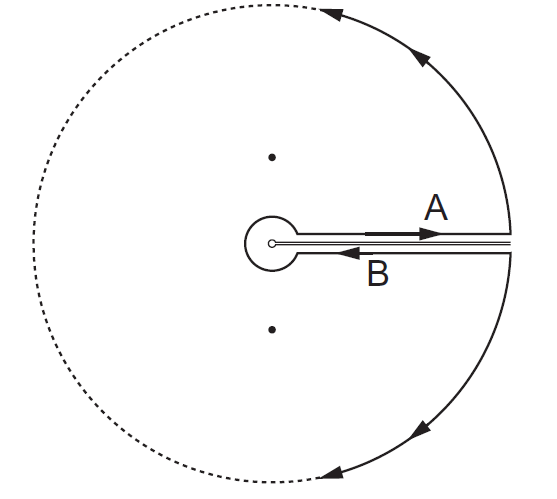
\includegraphics{2020/02/20200224_contour.PNG}
    \end{center}
    and see what this does for us.
    
    Note the poles marked here are for the previous example. Here, we have poles at $e^{\pi i/3},e^{\pi i}, e^{5\pi i /3}$ and we will need to evaluate the three residues. Now as before we get the integral over the upper segment $A$ and the lower segment $B$; $\ln x dx$ goes to zero quickly about the small circular region near the origin, and this integral goes away as $\ln x/x^2$ as $x\to \infty$. Hence our integral is
    \begin{equation}
        \oint = \int_0^\infty dx \frac{\ln x}{1+x^3} - \int_0^\infty dx \frac{\ln x +2\pi i}{1+x^3} = -2\pi i I,
    \end{equation}
    where $I$ is the integral we wanted. Since the contour integral is $2\pi i\times{}$ the residues, we find that
    \begin{equation}
        -I= \text{Res}_1 + \text{Res}_2 + \text{Res}_3.
    \end{equation}
    If we work it out, we find that
    \begin{equation}
        I= \frac{2\pi}{3\sqrt{3}},
    \end{equation}
    just as before.
\end{exm}
%It is a coincidence, but it is not an accidental coincidence.
%There are no dumb questions, there can only be dumb answers.

\begin{exm}
    Consider
    \begin{equation}
        \int_0^\infty dx \frac{x}{\sinh x}.
    \end{equation}
    The integrand is even, so we can extend it as
    \begin{equation}
        \frac{1}{2}\Int dx \frac{x}{\sinh x}.
    \end{equation}
    As $|x|$ grows large, the exponentials force this to converge. But how should we close the contour? The Jordan lemma doesn't apply. However, notice the following.
    \begin{equation}
        \sinh iy = \frac{1}{2} (e^{iy} -e^{-iy}) = i \sin y.
    \end{equation}
    Recall that $\sinh(x)$ follows the addition formula
    \begin{equation}
        \sinh(x+i\pi) = \sinh x \cosh (i\pi) + \cosh x \sinh (i\pi),
    \end{equation}
    so because $\sinh i\pi=i\sin \pi =0$ and $\cosh i\pi = \cos \pi =-1$, we find that
    \begin{equation}
        \sinh(x+i\pi) =-\sinh x.
    \end{equation}
    We see that $\sinh$ is $2\pi$-periodic in the imaginary direction. Therefore this suggests that we take a rectangular contour of height $i\pi$ and length $2L$. The sides are
    \begin{equation}
        \int_0^\pi i dy \frac{\pm L + iy}{\sinh(\pm L +iy)},
    \end{equation}
    which goes away as $L\to \infty$, so our integral is
    \begin{equation}
        \oint = \Int + \Int dx \frac{x +i\pi}{\sinh x}.
    \end{equation}
    If we treat the $\frac{i\pi}{\sinh x}$ as a principal value, we find that its principal value is zero. Hence
    \begin{equation}
        \oint =2\Int dx \frac{x}{\sinh x},
    \end{equation}
    and all we need to do is add the residues. This has a pole at $z=\pi i$, so when we take the residue we find that it is
    \begin{equation}
        \lim_{z\to \pi i} (z-\pi i) \frac{z}{\sinh z} =-\pi i
    \end{equation}
    and so
    \begin{equation}
        I= \frac{\pi^2}{4}.
    \end{equation}
\end{exm}
% \section{Wednesday, February 26, 2020}
%     Today we'll discuss using contour integrals to compute infinite sums. We'd like to sum a series like
\begin{equation}
    \sum_{n} a_n,
\end{equation}
and we want to write it in terms of a contour integral. Consider the function $\cot z = \frac{\cos z}{\sin z}$. The function $\sin z$ has the product expansion
\begin{equation}
    \sin z = z \prod_{n=1}^\infty \paren{1-\frac{z}{n\pi}} \paren{1+\frac{z}{n\pi}},
\end{equation}
so we have (nondegenerate) zeroes at integer $\pi$ and therefore $\cot z$ has simple poles at integer $\pi$.%
    \footnote{The degeneracy of a zero is easily counted by taking derivatives and evaluating the function at that zero until the net result is nonzero. For instance, $f(x)=(x-1)^2$ has a double zero at $x=1$. But $f(1)=0$ and $f'(1)=2(x-1)|_{x=1}=0$; only $f''(1)=2\neq 0$.}
Thus the residue at such poles is
\begin{equation}
    \lim_{z\to n\pi}(z-n\pi) \cot z = \frac{(z-n\pi)\cos z}{\sin z}.
\end{equation}
We can set a normalization so that $\cot \pi z$ has poles at integer $n$. Now consider the function
\begin{equation}
    f(z) \cot(\pi z),
\end{equation}
where $f(z)$ does not have any poles at real integer values. Suppose that $f(z)$ has some poles in the complex plane, however, at $\set{z_i}$. Then if we take the contour integral over a circle of radius $R$ centered on the origin and take $R\to \infty$, then
\begin{equation}
    \oint f(z) \cot (\pi z) dz = 2\pi i \sum_{n=-\infty}^\infty f(n) + 2\pi i \sum_{z_i} \text{Res} f(z)\cot \pi z.
\end{equation}
If $f$ decays sufficiently fast as $z\to \infty$, then the contour integral over the circle at infinity is zero, and we conclude that
\begin{equation}
    \sum_{n=-\infty}^\infty f(n) = -\sum_{z_i} \text{Res} f(z)\cot \pi z.
\end{equation}
\begin{exm}
    Suppose we wish to sum the series
    \begin{equation}
        S=\sum_{n=1}^\infty \frac{1}{n^2+a^2}.
    \end{equation}
    Notice that the summand is even in $n$, so
    \begin{equation}
        S= \sum_{n=-1}^\infty \frac{1}{n^2+a^2}.
    \end{equation}
    We can easily add on the $n=0$ term, which is just $1/a^2$. Thus
    \begin{equation}
        2S+\frac{1}{a} = \sum_{n=-\infty}^\infty \frac{1}{n^2+a^2},
    \end{equation}
    which is related to the contour integral
    \begin{equation}
        \oint_{C_R} dz\frac{1}{z^2+a^2} \cot(\pi z).
    \end{equation}
    This has poles everywhere we want, but it also has poles at $z=\pm ia$. So the value of this integral is
    \begin{equation}
        2\pi i \paren{\sum_{n=-\infty}^\infty \frac{1}{n^2+a^2} + 2\frac{\cot (\pi i a)}{2ia}}=0,
    \end{equation}
    and so
    \begin{equation}
        \sum_{-\infty}^\infty \frac{1}{n^2+a^2} = \frac{\pi}{a} \coth(\pi a).
    \end{equation}
\end{exm}
\begin{exm}
    Consider the sum
    \begin{equation}
        \sum_{n=1}^\infty \frac{1}{n(n+1)} = \sum_{n=1}^\infty \paren{\frac{1}{n}-\frac{1}{n+1}}.
    \end{equation}
    There's a somewhat pedestrian way to sum this series. If we take the partial sums $\sum_{n=1}^N$ then these sums are
    \begin{equation}
        1+ \frac{1}{2} + \frac{1}{3}+\dots + \frac{1}{N} - \paren{\frac{1}{2} + \frac{1}{3}+\dots + \frac{1}{N+1}}=1-\frac{1}{N+1},
    \end{equation}
    and as $N\to \infty$ we see the sum is just $1$.
    
    Let's do this a tricky way. By shifting $n\to -n$ and changing the index, we can see that
    \begin{equation}
        \sum_{n=-2}^\infty \frac{1}{n(n+1)}=\sum_{n=1}^\infty \frac{1}{n(n+1)},
    \end{equation}
    our original sum. We can almost extend this to the full infinite sum $\sum_{n=-\infty}^\infty$, but the $n=0$ and $n=-1$ terms are no good. We can write
    \begin{equation}
        2S= \sum_{-\infty}^\infty{}' \frac{1}{n(n+1)},
    \end{equation}
    where the prime indicates we must omit $n=0$ and $n=-1$. These are poles, which suggests that we have picked up double-poles at $n=0,n=-1$. That is,
    \begin{equation}
        0=\oint dz \frac{1}{z(z+1)} \cot \pi z.
    \end{equation}
    The residue at $z=0$ is the usual limit
    \begin{equation}
        \lim_{z\to 0} z^2 \cot \pi z
    \end{equation}
    and $z=-1$ is similar. Hence
    \begin{equation}
        \sum_{-\infty}^\infty{}' \frac{1}{n(n+1)} = -\text{Res}\paren{\frac{1}{z(z+1)}\cot(\pi z}_{z=0}-\text{Res}\paren{\frac{1}{z(z+1)}\cot(\pi z}_{z=-1}.
    \end{equation}
    This is precisely analogous to having dipoles rather than monopoles at some integer locations on the real line.
\end{exm}
%is 1/5 minus one sixth zero? Yes? No, it's 1/30!

\subsection*{Schwartz reflection principle}
The Schwartz reflection principle tells us how to take complex conjugates of various functions. We have seen previously that $f^*(z)= f(z^*)$, but in fact there are conditions. Consider
\begin{equation}
    \bkt{(z-x_0)^n}^* = (z^*-x_0)^n,
\end{equation}
where $x_0\in \RR$. When we take linear combinations $\sum a_n(z-z_0)^n$, we might have to complex conjugate the $a_n$s as well. The Schwartz reflection principle provides sufficient conditions so this does not happen.

Consider $f(z)$ analytic. Hence we can Taylor expand $f$ about a point $x_0$ on the real line,
\begin{equation}
    f(z) = \sum \frac{f^{(N)}(x_0)}{n!}(z-x_0)^n,
\end{equation}
where $z_0$ is real. Moreover, suppose that for real arguments $x_0\in \RR$, $f^*(x_0)=f(x_0)$, i.e. $f$ is real-valued for real arguments. Hence all the $f^{(n)}(x_0)$ are also real. This must be the case since the $(z-x_0)^n$ factors are all linearly independent. Hence
\begin{equation}
    f^*(z) = \sum \frac{f^{(n)}(x_0)}{n!}(z^*-x_0)^n = f(z^*).
\end{equation}



% % week 9
% \section{Monday, March 2, 2020}
% 	\begin{quote}
    \textit{``Any of you who take the bold and foolish step of getting lost in theory will become familiar with these things [Fourier-transformed Gaussians].''}
    
    ---Nemanja Kaloper
\end{quote}
Last time, we defined the Fourier transform
\begin{equation}
    g(k) = \Int \frac{dx}{\sqrt{2\pi}}f(x) e^{-ikx}
\end{equation}
and the inverse transform%
    \footnote{It's a matter of convention whether we decide to put the $\sqrt{2\pi}$s in both the normal and inverse transform, or whether we put e.g. the $1/2\pi$ with the inverse transform. In QFT I usually write $d^dk/(2\pi)^d$ and put the $2\pi$s with the inverse transform when I take $dk$ integrals, where $d$ is the dimension we're working in (often in e.g. $d=4$) but there's not a lot of difference.}
\begin{equation}
    f(x) = \Int \frac{dk}{\sqrt{2\pi}} g(k) e^{ikx},
\end{equation}
such that the completeness relations
\begin{align}
    \Int dx \,e^{ik(x-x')}&=2\pi \delta(x-x'),\\
    \Int dx \,e^{i(k-q)x} &= 2\pi \delta(k-q)
\end{align}
hold. This uses the convention that $e^{i\omega t}$ is the time dependence of a positive-frequency wave moving forward in time.

Suppose $f(x)$ has definite parity, e.g. $f$ is even, $f(-x)=f(x)$. Then we can just do the integral over the half-line and write
\begin{align*}
    g(k) &= \int_0^\infty \frac{dx}{\sqrt{2\pi}}f(x) e^{-ikx} + \int_0^\infty \frac{dx}{\sqrt{2\pi}}f(x)e^{+ikx}\\
        &= \sqrt{\frac{2}{\pi}} \int_0^\infty dx\, f(x) \cos(kx).
\end{align*}
This is the \emph{even Fourier transform.} By an equivalent argument, if our function is instead odd, then
\begin{equation}
    \tilde g(k) = \sqrt{\frac{2}{\pi}} \int_0^\infty dx\, f(x) \sin(kx),
\end{equation}
where the tilde indicates we have dropped a factor of $i$ in going from exponentials to a sine.

\begin{exm}
    Take the function $f(x) = e^{-\alpha|x|}$, with $\alpha >0$. Then
    \begin{align*}
        g(k) &= \frac{1}{\sqrt{2\pi}}\int_0^\infty dk \, e^{-\alpha x} e^{-ikx} + \frac{1}{\sqrt{2\pi}} \int_0^\infty dx \, e^{-\alpha x} e^{+ikx}\\
            %&= \frac{1}{\sqrt{2\pi}} \bkt{\frac{e^{-(\alpha + ik)x}}{-(\alpha + ik)}}_0^\infty
            &= \frac{1}{\sqrt{2\pi}} \bkt{\frac{1}{\alpha+ik} +\frac{1}{\alpha-ik}}\\
            &= \sqrt{\frac{2}{\pi}} \frac{\alpha}{\alpha^2 + k^2}.
    \end{align*}
\end{exm}
We can easily take the Fourier transform of a delta function as well, $\delta(x)$. Well,
\begin{equation}
    g^\delta(x) = \frac{1}{\sqrt{2\pi}}.
\end{equation}
The fact that the Fourier transform is constant in momentum space tells us that if we want to build a completely localized wavepacket in position space, we need to use components of all frequencies in momentum space.
%a Weinberg, S HEP InSpire

\begin{exm}
    Now let us show that the inverse transform gives back the original function using $f(x)=e^{-\alpha|x|}$. We write the transformed function as
    \begin{equation}
        \sqrt{\frac{2}{\pi}} \frac{k}{x^2+k^2},
    \end{equation}
    and now
    \begin{equation}
        \frac{k}{\pi} \Int dx \frac{e^{ik'x}}{x^2+k^2}
    \end{equation}
    is our original function. But which way we close the contour clearly depends on the sign of $k$. For $k>0$ we should close it in the lower half-plane, so
    \begin{equation}
        \frac{k}{\pi} \Int dx \frac{e^{-ikx}}{(x-ik)(x+ik)} = \frac{k}{\pi} \paren{2\pi i \frac{e^{-ik(-ik)}}{(-2ik)}} = e^{-k' k}.
    \end{equation}
\end{exm}

%Any of you who take the bold and foolish step of getting lost in theory will become familiar with these things [Fourier-transformed Gaussians].

\begin{exm}
    Let's take the Fourier transform of a Gaussian. That is,
    \begin{equation}
        f(x) = e^{-\alpha x^2}
    \end{equation}
    so that the transform is
    \begin{align*}
        g(k) &= \frac{1}{\sqrt{2\pi}} \Int dx\, e^{-\alpha (x^2 +ik/\alpha)}\\
            &= \frac{1}{\sqrt{2\pi}} \Int dx \, e^{-\alpha\paren{[x+ik/2\alpha]^2 + k^2/4\alpha^2}}.
    \end{align*}
    THe $k^2/4\alpha^2$ term is constant-- it does not depend on $x$. The rest is a Gaussian, but with a complex shift:
    \begin{equation}
        g(k) = \frac{e^{-k^2/4\alpha}}{\sqrt{2\pi}}\Int dx\, e^{-\alpha [x+ik/2\alpha]^2}.
    \end{equation}
    Now we can make a change of variables to write
    \begin{equation}
        g(x) = \frac{e^{-k^2/4\alpha}}{\sqrt{2\pi}}\int_{-\infty +ik/2\alpha}^{+\infty + ik/2\alpha} d\hat x e^{-\alpha \hat x^2}.
    \end{equation}
    This isn't quite our original Gaussian integral because it is not over the real line yet, and we'd very much like to use the result $\Int e^{-\alpha x^2}=\sqrt{\pi/\alpha}.$
    
    We can relate this to the integral over the real line, however, by taking a rectangular contour of length $2L$ and height $ik/2\alpha$. The sides are exponentially suppressed as we take $L\to \infty$, and there are no poles in the rectangular contour, so the integral over the line $x+ik/2\alpha$ is equal to the integral over the real line, $x\in \RR$.
    
    It follows that this integral really is our Gaussian integral, so the result is
    \begin{equation}
        g(k) = \frac{e^{-k^2/4\alpha}}{\sqrt{2\alpha}}.
    \end{equation}
    As it turns out, the Fourier transform is another Gaussian, but with a different width of $\sqrt{2\alpha}$ rather than $1/\sqrt{\alpha}$.
\end{exm}

\begin{exm}
    Suppose we have a sine wave which is only on for some finite pulse,
    \begin{equation}
        f(x) = \begin{dcases}
            \sin (\omega_0 t) & |t| < \frac{N\pi}{\omega_0},\\
            0 & |t| > \frac{N\pi}{\omega_0}.
        \end{dcases}
    \end{equation}
    This is an odd function, so we can compute
    \begin{equation}
        \sqrt{\frac{2}{\pi}}\int_0^{N\pi/\omega_0}dt \sin(\omega_0 t) \sin(\omega t).
    \end{equation}
    Now we can use trig addition formulae to turn the product of sines into regular cosines:
    \begin{equation}
        \sin\alpha \sin \beta = \frac{1}{2}[\cos(\alpha-\beta) -\cos(\alpha+\beta)].
    \end{equation}
    If we put the pieces together and do the integral, we get
    \begin{equation}
        \frac{1}{\sqrt{2\pi}}\paren{\frac{\sin\bkt{(\omega_0 - \omega)(N\pi/\omega_0)}}{\omega_0-\omega} - \frac{\sin\bkt{(\omega_0+\omega) (N\pi/\omega_0)}}{\omega_0+\omega}}
    \end{equation}
    This function has a resonance at $\omega = \omega_0$. The next peak is when $(\omega_0-\omega)(N\pi/\omega_0) = \pi/2$, so the distance to the next peak is $\delta \omega = \omega_0/N$. It follows that $\Delta \omega \Delta t=\pi$, i.e. the spacing between peaks in frequency space and the spacing between peaks in time is constant.
\end{exm}

% \section{Wednesday, March 4, 2020}
%     \begin{quote}
    \textit{``I like all things if they're valuable, okay? I collect them.''}
    
    ---Nemanja Kaloper
\end{quote}

Building off last time, we can define 3-dimensional equivalents of the Fourier transform,
\begin{equation}
    f(\vec x) = \int \frac{d^d\vec k}{(2\pi)^{d/2}}g(\vec k) e^{-i\vec k \vec x}
\end{equation}
and
\begin{equation}
    g(\vec k) = \int \frac{d^d\vec x}{(2\pi)^{d/2}}f(\vec x) e^{i\vec k \cdot \vec x}.
\end{equation}

\begin{exm}
    Consider the Yukawa potential,
    \begin{equation}
        f(r) = \frac{e^{-\alpha r}}{r}=\frac{e^{-r/m}}{r},
    \end{equation}
    where $\alpha=m >0$. We may do this in order to ensure convergence. Consider now its Fourier transform,
    \begin{equation}
        \int d^3x \frac{e^{-\alpha|\vec x|}}{|\vec x|} e^{-i|\vec k| |\vec x| \cos \theta}.
    \end{equation}
    Since we integrate over all space and all angles, WLOG we can take $\vec k$ to point along the $\uv z$ direction in order to perform the integral. Notice that this integral retains an azimuthal symmetry, so it's most natural to transform to spherical coordinates. This integral becomes
    \begin{equation}
        2\pi \int_0^\infty dr r^2 \int_0^\pi d\theta \sin\theta \frac{e^{-\alpha|\vec x|}}{|\vec x|} e^{-i|\vec k| |\vec x| \cos \theta}.
    \end{equation}
    The book resorts to expanding in spherical harmonics, but there's really no need to do it. We have $d\sin\theta = d(-\cos\theta)$ so the angular integral is easy to do. Our integral simplifies to
    \begin{align*}
        g(\vec k) &= 2\pi \int_0^\infty dr \, re^{-\alpha r} \int_{-1}^1 d(\cos\theta) e^{-ikr(\cos\theta)}\\
            &= \frac{2\pi i}{k} \int_0^\infty dr\, e^{-\alpha r} \paren{e^{-ikr} - e^{+ikr}}\\
            &= \frac{2\pi i}{k} \int_0^\infty dr \paren{e^{-(\alpha +ik)r} - e^{-(\alpha-ik)r}}.
    \end{align*}
    This last expression is similar to what we computed last time. The $e^{\pm ikr}$ phase doesn't affect convergence, since $e^{-\alpha r}|e^{ikr}|$ converges absolutely. Thus
    \begin{equation}
        g(k) = \frac{2\pi i}{k} \bkt{\frac{1}{\alpha+ik} - \frac{1}{\alpha-ik}} = \frac{2\pi i}{k} \frac{-2ik}{\alpha^2+k^2} = \frac{4\pi}{\alpha^2+k^2}.
    \end{equation}
    The Fourier transform of the Yukawa potential has turned out to be a Lorentzian in $k$-space.%
        \footnote{See \url{http://mathworld.wolfram.com/LorentzianFunction.html}.}
    However, note that if the mass is zero, we lose the factor $e^{-\alpha|\vec x|}$ which gave us convergence. What happens now? Our integral becomes
    \begin{equation}
        \frac{2\pi i}{k} \int_0^\infty dr \paren{e^{-ikr} - e^{+ikr}} = -\frac{2\pi i}{k} \paren{\int_0^L + \int_0^{-L}}dr e^{ikr}.
    \end{equation}
    The lower limit gives us the correct answer, but we have to understand the behavior at infinity. Inserting the regularizing factor $e^{-\alpha|x|}$ allows us to actually cut off the behavior at infinity (at large distances $x$) and then take the $\alpha\to 0$ limit.
    
    Hence we we can say that (restoring factors of $2\pi$)
    \begin{equation}
        g(k) = \frac{1}{(2\pi)^{3/2}} \frac{4\pi}{\alpha^2 +k^2}
    \end{equation}
    and in the $\alpha\to 0$ limit,
    \begin{equation}
        g(k) \to \frac{1}{(2\pi)^{3/2}} \frac{4\pi}{k^2}.
    \end{equation}
    Let us take the inverse transform and confirm that it all works out. That is, we shall integrate
    \begin{align*}
        \int d^3x \frac{e^{-i|\vec k||\vec x|\cos\theta}}{|\vec x|^2} &= 2\pi \int_0^\infty dr \int_{-1}^1 d(\cos\theta) e^{-ikr(\cos\theta)}\\
            &= \frac{2\pi i}{k} \int_0^\infty dr \frac{1}{r} \paren{e^{-ikr} - e^{ikr}}\\
            &= -\frac{2\pi i}{k} \int_0^\infty \frac{dr}{r} \paren{e^{+ikr} - e^{-ikr}}.
    \end{align*}
    Now we can flip the sign in the exponent of the second term and get
    \begin{equation}
        -\frac{2\pi i}{k} \bkt{\int_0^\infty \frac{dr}{r} e^{ikr} - \int_0^{-\infty} \frac{dr}{r} e^{+ikr}},
    \end{equation}
    which we recognize as a single principal value integral,
    \begin{equation}
        -\frac{2\pi i}{k} \Int \frac{dr}{r} e^{ikr}.
    \end{equation}
    Moreover the combination $dr/r$ is scale-invariant, as are the limits of integration, so we can reparametrize to $\Int \frac{dz}{z} e^{-iz}.$ Performing the integral gives us our final answer,
    \begin{equation}
        \frac{4\pi^2}{k},
    \end{equation}
    which upon restoring $2\pi$s gives us our original Coulombic potential as promised.
\end{exm}

Let's mention some properties of the Fourier transform. If we have a function $f(\vec x)$, let us denote its Fourier transform as
\begin{equation}
    \bkt{f(\vec x)}^T = \frac{1}{(2\pi)^{3/2}}\int d^3 \vec x e^{i\vec k \cdot \vec x}.
\end{equation}
Then the Fourier transform of the shifted function is
\begin{equation}
    \bkt{f(\vec r- \vec R}^T = e^{i\vec k \cdot \vec R} g(\vec k).
\end{equation}
Similarly the Fourier transform of the rescaled argument is
\begin{equation}
    \bkt{f(\alpha \vec r)}^T = \frac{1}{\alpha^3} g\paren{\frac{\vec k}{\alpha}},
\end{equation}
where the overall scaling factor comes from the integration measure $d^3x$. Inversion gives
\begin{equation}
    \bkt{f(-\vec r)}^T = g(-\vec k),
\end{equation}
setting $\alpha =-1$. Note there's no overall minus sign because both the measure and the limits of integration flip. Complex conjugation and inversion gives
\begin{equation}
    \bkt{f^*(-\vec r)}^T = g^*(\vec k),
\end{equation}
while taking a derivative brings down an $ik$:
\begin{equation}
    \bkt{\grad f(\vec r)}^T = -i\vec k g(\vec k),
\end{equation}
and doing the Laplacian gives
\begin{equation}
    \bkt{\nabla^2 f(\vec x)}^T = -k^2 g(\vec k).
\end{equation}

%I like all things if they're valuable, okay? I collect them.
%Imagine two guys sitting in two boats on a lake throwing snowballs at each other.

% % week 10
% \section{Monday, March 9, 2020}
% 	%The reason we joined Costco was because of diapers. Kids can be quite productive, shall we say.
Today we'll continue our discussion of convolutions (Faltung). The convolution was defined as
\begin{equation}
    f*g = \Int \frac{dy}{\sqrt{2\pi}} g(y) f(x-y) = \int \frac{dk}{\sqrt{2\pi}} G(k) F(k) e^{-ikx},
\end{equation}
where $F$ and $G$ are the Fourier transforms of $f$ and $g$ respectively. In particular, if we take $x=0$ then we get the result known as the Parseval relation,
\begin{equation}
    \int dy\, g(y) f(-y) = \int dk G(k) F(k).
\end{equation}
This almost looks like an overlap integral, but we can rewrite a bit. Let us define a function $\hat f(y)$ such that
\begin{equation}
    \hat f^*(-y) = f(y).
\end{equation}
Then its Fourier transform $\hat F$ is just the complex conjugate of $F$, i.e.
\begin{equation}
    F(k) = \bkt{f(y)}^T = \bkt{\hat f^*(-y)}^T = \hat F^*(k).
\end{equation}
Thus
\begin{equation}
    \braket{\hat f}{g} = \int dy\, \hat f^*(y) g(y)  = \int dk \hat F^*(k) G(k) = \braket{\hat F}{G}.
\end{equation}
We find that the Fourier transform is unitary; it preserves the inner product on the space of square integrable functions. That is,
\begin{equation}
    \braket{f}{g} = \braket{F}{G} = \braket{Uf}{Ug}
\end{equation}
for $F=Uf$, where we've written the Fourier transform as a (linear) operator $U$ on functions (vectors in a Hilbert space). In other words, going from coordinate (position) space to momentum space is just a unitary transformation.

Now suppose we have an equation we wish to solve,
\begin{equation}
    \cL y=J
\end{equation}
for $\cL$ some differential operator. Then
\begin{equation}
    y(x) = \Int J(y) G(x-y) dy = \int dk \,G^T(k) J^T(k) e^{-ikx}.
\end{equation}
That is, we can determine the Green's function for an operator (given appropriate boundary conditions) and then Fourier transform the convolution integral required to solve the inhomogeneous equation.

For instance, we can write an electrostatic potential as
\begin{equation}
    \psi(\vec r) = \frac{1}{4\pi} \int d^3 r' \frac{\rho(\vec r')}{|\vec r- \vec r'|} = \frac{1}{(2\pi)^{3/2}}\int d^3 k \frac{\rho^T(k)}{k^2} e^{-i\vec k \cdot \vec r}.
\end{equation}
This gives us the electrostatic potential in terms of the Fourier transform of the charge distribution.

We can define multiple convolutions as well.
\begin{align*}
    (f*(g*h))(x) &= \int \frac{dy}{\sqrt{2\pi}}(g*h)(y) f(x-y)\\
        &= \int \frac{dy}{\sqrt{2\pi}} f(x-y) \int \frac{dz}{\sqrt{2\pi}} h(z) g(y-z)\\
        &= \int \frac{d\tilde y}{\sqrt{2\pi}} \frac{dz}{\sqrt{2\pi}} f(\tilde y) g(\tilde y-z-x) h(z)
\end{align*}
with $\tilde y = x-y$. Equivalently we could use $\tilde z = y-z$ and write this as
\begin{equation}
    \int \frac{d\tilde y}{\sqrt{2\pi}} \frac{d\tilde z}{\sqrt{2\pi}} f(\tilde y) g(\tilde z) h(x-\tilde y - \tilde z).
\end{equation}
It follows that convolution is associative, and moreover one can show that $f*g=g*f$, so convolution gives a commutative algebra.

For the electrostatic potential
\begin{equation}
    \psi(\vec r) = \frac{1}{4\pi} \int d^3 r' \frac{\rho(\vec r')}{|\vec r- \vec r'|},
\end{equation}
the interaction energy of two charge distributions is
\begin{align*}
    W &= \int d^3 r \, \rho(\vec r) \psi(\vec r) \\
        &= \frac{1}{4\pi} \int d^3r \, d^3 r' \, \rho(\vec r) \frac{1}{|\vec r- \vec r'|} \rho(\vec r').
\end{align*}
Now we recognize this as a convolution integral and write this in terms of the Fourier transforms to find that
\begin{equation}
    W= 4\pi \int d^3 k\, d^3 k'\, \rho^T(\vec k) \frac{1}{k^2} \rho^T(-\vec k').
\end{equation}
In a sense, the relation
\begin{equation}
    [g*f]^T = F(k) G(k)
\end{equation}
defines the Fourier transform. Conversely
\begin{equation}
    [F*G]^T = fg.
\end{equation}
That is, a convolution in one space becomes a product in the Fourier-transformed space. Notice that the converse is not exactly true:
\begin{equation}
    [fg]^T = F*G \text{ \emph{if $F$ and $G$ exist.}}
\end{equation}
Sometimes $F$ does not exist, but $f$ may have a Taylor expansion and we can write the Fourier transform of a product order-by-order for some $\sum a_n [x^n g]^T$. Moreover we know that multiplying by $x$ corresponds to taking $i\P{}{k}$ derivatives of the Fourier transform. That is, if $f$ has a Taylor series, then
\begin{equation}
    [f(x)g]^T = \sum a_k \paren{i\P{}{k}}^n g^T(k) = f\paren{i\P{}{k}} g^T(k).
\end{equation}
We can thereby make sense of expressions like
\begin{equation}
    \frac{1}{z-D} = \frac{1}{z} \frac{1}{1-\frac{1}{z}D} = \frac{1}{z} \sum \paren{\frac{1}{z}D}^n,
\end{equation}
and we recognize that the inverse of a derivative is of course an integral, so an integral can in a sense be written as an infinite sum of derivatives.

Our aim in much of this is often to solve the Schr\"odinger equation,
\begin{equation}
    \bkt{\frac{\hat p^2}{2m} + V(x)}\ket{\psi} = E \ket{\psi}.
\end{equation}
Notice we can rewrite as
\begin{equation}
    \bkt{\frac{p^2}{2m} + V(i\grad_{\vec p})} \psi^T(\vec p) = E \psi^T(p).
\end{equation}
In general this might be harder to solve than the original equation, depending on how nasty $V(x)$ is. But for the harmonic oscillator (rescaled so $m=1$ and $\omega=1$) takes a very simple form:
\begin{equation}
    \bkt{\frac{p^2}{2} + \frac{x^2}{2}}\psi = E \psi,
\end{equation}
which is now manifestly symmetric in $x$ and $p$ so that the equation in Fourier space looks exactly the same as it did in position space. We work in coordinate space because things appear to be localized in position space, but from a theoretical/calculational perspective either is perfectly good.which is now manifestly symmetric in $x$ and $p$ so that the equation in Fourier space looks exactly the same as it did in position space. We work in coordinate space because things appear to be localized in position space, but from a theoretical/calculational perspective either is perfectly good.


% \section{Wednesday, March 11, 2020}
%     We have options for the final.
-no final
-regular 2 hour exam plus 30 mins for formatting and submission
-``long homework'' (48 hours)

%In the end it's never me who grades you, it's you yourself.

\subsection*{Legendre polynomials, revisited}

Let us recall that Legendre polynomials are a complete set of functions which solve the differential equation
\begin{equation}
    (1-x^2)P''(x)+2xP'(x) + \lambda P(x)=0.
\end{equation}
For generic $\lambda$, power series (Frobenius) expansions do not terminate, except for special values of $\lambda$ such that
\begin{equation}
    \lambda = l(l+1), \quad l = 0,1,2,\dots
\end{equation}
and we label the solutions as $P_l(x)$. We also saw the Legendre polynomials when we were solving differential equations with spherical symmetry. The Legendre polynomials emerge when we write the Laplacian in spherical coordinates and attempt to solve the Poisson/Laplace equations.

Consider the equation
\begin{equation}
    \Delta \psi = q\delta(\vec r- \vec r').
\end{equation}
This has the Coulomb form of the potential,
\begin{equation}
    \psi(\vec r) = \frac{1}{|\vec r - \vec r'|} = \frac{1}{\sqrt{r^2-r r' \cos\theta + r'^2}}.
\end{equation}
If the point of interest $\vec r$ is much farther away from the origin than the point charge, $|\vec r|>|\vec r'|$, then we can write
\begin{equation}
    \psi(\vec r) =\frac{1}{r} \frac{1}{1-2tx +t^2} = \frac{1}{r} \sum_{n=0}^\infty P_n(x) t^n,
\end{equation}
where we have defined
\begin{equation}
    t= \frac{r'}{r} <1, \quad  x = \cos\theta.
\end{equation}
This is an exterior spherical expansion. Notice that the identity
\begin{equation}
    \frac{1}{1-2tx +t^2} = \sum_{n=0}^\infty P_n(x) t^n
\end{equation}
therefore tells us all the Legendre polynomials---we need only to expand in powers of $t$ and collect their coefficients in $x$. We call this a \term{generating function} for the Legendre polynomials. There exist also associated Legendre polynomials, which are related to the usual ones by derivatives.%
    \footnote{There's a paper in Reviews of Modern Physics by Bander and Itzyckson on properties of the Legendre polynomials and spherical harmonics.}
One can also analytically continue the argument of the Legendre polynomials, depending on what one is interested in. There's a generating function for Bessel functions, too:
\begin{equation}
    e^{-\frac{x}{2}(z- \frac{1}{z})} = \sum_{n=-\infty}^\infty J_n(x) z^n.
\end{equation}
Generating functions are useful because they reveal certain commonalities between all the special functions in a family, e.g. special values. For instance, what is $P_n(x=\pm 1)$? Well,
\begin{equation}
    \sum_{n=0}^\infty P_n(x=\pm 1) t^n =\frac{1}{\sqrt{1-2(\pm 1)t +t^2}} = \frac{1}{1\mp t}.
\end{equation}
We can Taylor expand now.
\begin{equation}
    \frac{1}{1-t} = \sum t^n, \quad \frac{1}{1+t} = \sum (-1)^n t^n,
\end{equation}
and that immediately gives us
\begin{equation}
    P_n(x=\pm 1) = (\pm 1)^n.
\end{equation}
We can calculate the value at $x=0$ too:
\begin{equation}
    \sum_{n=0}^\infty P_n(x=0)t^n = \frac{1}{\sqrt{1+t^2}}.
\end{equation}
One finds that
\begin{equation}
    P_n(0) = \begin{dcases}
        0 & n = 2l+1\\
        \frac{1}{(2n)!} D^{2n}(1+t^2)^{-1} & \text{otherwise}
    \end{dcases}
\end{equation}
since there are no odd powers of $t$ in the Taylor expansion. This derivative turns out to be $\binom{-1/2}{n} = (-1)^n \frac{(2n-1)!!}{(2n)!!}$.
Equivalently one may write
\begin{equation}
    \frac{1}{\sqrt{1-2xt+t^2}}= (1-z)^{-1/2} = \sum_{n=0}^\infty \binom{-1/2}{n}(-2xt + t^2)^n
\end{equation}
in a binomial expansion. %For notice that at order $x^k$ we have terms like $(xt)^k t^{2(n-k)}$

Now, we claimed that the generating function somehow knows about all the properties of the Legendre polynomials. That suggests it should have a link to the differential equation. Well, suppose we derive the sum expression by $t$. We get
\begin{equation}
    \sum_{n=0}^\infty n P_n(x) t^{n-1} = \sum_{n=0}^\infty (n+1) P_{n+1}(x) t^n,
\end{equation}
and the derivative of the square root expression is
\begin{equation}
    \frac{d}{dt}\frac{1}{\sqrt{1-2xt+t^2}} = \frac{x-t}{(1-2xt+t^2)^{3/2}} = \frac{x-t}{\sqrt{1-2xt+t^2}(1-2x+t^2)}.
\end{equation}
It follows that
\begin{equation}
    (1-2xt +t^2) \sum_{n=0}^\infty (n+1) P_{n+1}(x) t^n = (x-t) \sum_{n=0}^\infty P_n(x) t^n,
\end{equation}
where we have recognized and expanded the square root using the generating function. If we count order by order in $t$, we recover a recursion relation on the $P_n$:
\begin{equation}
    (2n+1) x P_n(x) =(n+1) P_n(x) + n P_{n-1}(x).
\end{equation}

This is not the only recursion relation we can find. We can also find one with derivatives with respect to $x$, i.e.
\begin{equation}
    \sum P_n'(x) t^n = \frac{d}{dx} \bkt{\frac{1}{\sqrt{1-2xt + t^2}}}.
\end{equation}
Taking the derivative and comparing by orders of $t$ again yields
\begin{equation}
    P_{n+1}'(x) + P_{n-1}'(x) = 2x P_n' + P_n,
\end{equation}
a recursion relation between derivatives of Legendre polynomials. This may not look pretty, but in fact it's a direct consequence of symmetry. The relations come from representations of Lie algebras.

\end{document}